\documentclass{article}
\usepackage[utf8x]{inputenc} 
\usepackage[english]{babel}
\usepackage{natbib}
\usepackage{booktabs}
\usepackage{setspace}\doublespacing
\setlength{\parskip}{0.5em}
\usepackage[left]{lineno}\linenumbers
\usepackage[a4paper, total={6in, 8in}]{geometry}
\usepackage{isomath}
\usepackage{amsmath}
\usepackage{mathtools}
\usepackage{longtable}
\usepackage[font={footnotesize,it}]{caption}
\usepackage{floatrow}
 
\usepackage[colorinlistoftodos]{todonotes}
\floatsetup[table]{capposition=top}


\begin{document}

\begin{center}
\large
\textbf{Social effects on fitness and the eco-evolutionary dynamics of populations: from density regulation to frequency-dependent selection}
\end{center}

\begin{center}
	Yimen G. Araya-Ajoy\textsuperscript{1,2}, Myranda Murray\textsuperscript{1},  Bernt-Erik Sæther\textsuperscript{1}, Jonathan Wright\textsuperscript{1}
\end{center}

\bigskip
\textbf{1} Centre for Biodiversity Dynamics (CBD), Department of Biology, Norwegian University of Science and Technology (NTNU), N-7491 Trondheim, Norway.

\bigskip
\textbf{2} Corresponding author, email address: yimencr@gmail.com

\bigskip
\textbf{Keywords}: density-dependent selection, multiple regression models, individual-based simulations, social selection gradients, social evolution

\newpage
\section{Abstract}
Social interactions are key determinants of the equilibrium density and mean phenotype of populations. Density regulation and frequency-dependent selection can be seen as two extremes of a continuum of effects of social interactions on the eco-evolutionary dynamics of populations. This continuum  describes how much the effect an individual has on the fitness of others depends upon its phenotype, and how much the effects on fitness an individual experiences due to intraspecific competition depends upon its own phenotype. We use individual-based models to simulate scenarios along this continuum, and analyze the outcomes using a set of multiple regressions designed to disentangle social effects causing temporal variation in population mean fitness from those causing individual differences in fitness. We discuss the links between these different statistical estimates and existing theory concerning the socio-ecological factors determining the equilibrium size and mean phenotype of populations. This study aims to stimulate more focused empirical research by connecting specific theoretical components of eco-evolutionary dynamics to standard statistical analyses that allow estimating the different social processes affecting population growth and evolutionary change. 

\newpage
\section{Introduction}
 The realization that evolutionary change can affect ecological and demographic processes over relatively short timescales has encouraged theoreticians to develop evolutionary models that explicitly take into account the feedback between population dynamics and phenotypic evolution \citep{Govaert2019, hendry2016eco}. This framework has provided many insights into the density-dependent feedbacks determining the links between the equilibrium size of populations and their equilibrium mean phenotype \citep{MacArthur1962, Charlesworth1994, Lande2009a, Engen2013, Engen2020}. Surprisingly, even though social behaviors are major drivers of the competitive and cooperative interactions driving density regulation and phenotypic selection, key components of classic theory on the evolution of social behavior have not been fully integrated into the eco-evolutionary paradigm. Social evolution theory has a very well developed analytical framework focusing upon the evolutionary dynamics of phenotypes mediating social interactions \citep{frank1998foundations, Wolf1999SocialSelection, Queller1985a, Queller2017, Araya-Ajoy2020}. However, within this framework it is often assumed that the population size is fixed, and thus for simplicity that the evolutionary dynamics of social interactions do not affect the size of populations and  \textit{vice versa}. Integrating components from these different approaches within a statistical framework allowing the quantification of evolutionary change and population growth will improve our empirical understanding of the eco-evolutionary dynamics of wild populations.

 Figure 1 depicts the role of social interactions in mediating eco-evolutionary feedbacks through density and frequency dependent processes \citep{Engen2020}. Path 1 (p1) shows how the strength of competition for limited resources determines population size through density regulation \citep{Gilpin1973a}. Change in population size in turn affects density-dependent competition (p2), creating the classic ecological feedback (p1,2) determining the equilibrium size of a population \citep{Travis2013}. If selection is density-dependent (p1,2,3), the size of a population will also have cascading effects on phenotypic selection  \citep{Mueller1997, Boyce1984}. For instance, when populations are large and closer to carrying capacity, investing in somatic growth and competitive behaviours to monopolize resources may be favored. In contrast, when populations are small and resources are abundant, selection may favor smaller individuals that invest in rapid reproduction instead of body size and longer-term competitive ability \citep{Joshi2001, Wright2018, Engen2017}. Density-dependent selection may thus result in the optimal phenotype being dependent upon population size \citep{Anderson1971, Charlesworth1971}. Evolutionary adjustments in the population mean phenotype can, in turn, influence the strength of competitive interactions via the relative frequencies of different phenotypes in the population \citep{Wright1969} (p4,1). Following the example of body size, as competition increases the average individual becomes bigger and needs more resources, thus reducing the maximum possible size of the population \citep{Engen2020}. However, if interacting individuals are genetically related, evolution may favor social strategies that maximize efficiency of resource use in order to ameliorate the negative fitness effects of kin competition, potentially increasing the carrying capacity of such populations \citep{Boyce1984, macarthur1967theory}. The average phenotype and genotype in the population can thus influence the optimal phenotype for a given individual, causing frequency-dependent selection to further affect phenotypic evolution (p4,3) \citep{Heino1998} and population size (p4,3,1) \citep{Svensson2018}. Social interactions thus mediate the feedback between ecological and evolutionary dynamics, linking the evolutionarily stable phenotype and the equilibrium size of a population (p5).

Social phenotypes have the potential to affect population dynamics and/or phenotypic evolution whenever the fitness of an individual is affected by other individuals in the same population. Indeed, we can imagine a continuum stretching between two conceptual extremes of social fitness effects (Figure 2). At one end we can envision density regulation (from population ecology, Figure 2A) where the effects of density on the mean fitness of a population are assumed to be independent of individual phenotypes. Whilst at the other end lies frequency-dependent selection (from evolutionary game theory) where the average phenotype in the population affects the relative fitness of different phenotypes in the population (Figure 2H). Most effects of social interactions on the eco-evolutionary dynamics of populations lie somewhere between these two extremes, whenever the impact an individual has on the fitness of others depends upon its phenotype and/or the changes in relative fitness that an individual experiences due to social interactions depend upon its own phenotype. The link between the equilibrium mean phenotype and the equilibrium population size, therefore depends upon how social traits moderate the effects of population size on fitness. A key aspect of evolution of social traits is that the drivers of selection can also evolve (e.g phenotypes in the social environment) \citep{West-Eberhard1979, Moore1997}. The evolution of the social environment, in the context off frequency- and density-dependent selection, will have cascading effects on density regulation and population dynamics, further affecting the evolution of social traits \citep{Heino1998}. The eco-evolutionary feedbacks caused by density- and/or frequency-dependent effects are thus determined by how social phenotypes influence the impact that individuals have on the fitness of others and/or how an individual's phenotype moderate the effect of population density on its own fitness \citep{Engen2020}. 

We here define social traits as phenotypes that have fitness effects on individuals other than the actor. The evolutionary consequences of such phenotypes  (Figures 2C and D) is the focus of the quantitative genetics theory on social evolution \citep{frank1998foundations, Araya-Ajoy2020}. A key component of this theory is social selection. Social selection gradients usually quantify the effect of the phenotypes in the social environment on the relative fitness of an individual within a given breeding episode \citep{Wolf1999SocialSelection} - shown as dashed lines in Figure 2D. In this context, it is assumed that social fitness effects influence evolutionary changes in the mean phenotype in the population, but they do not affect the growth of populations. Similar to 'soft' selection, this type of social selection has no effect on the mean fitness of the population \citep{Goodnight1992}, and thus no consequences in terms of variation in population size (Figure 2D). However, the phenotypic effects of an individual on the survival and reproduction of others can influence the mean fitness of the population (shown as black dots in Figure 2C) in a similar way to density regulation (Figures 2A). The effect of the phenotype of the average individual in the population on the absolute fitness of other individuals is expected to affect the mean fitness in the population. Such 'hard' social selection will partly define the relationship between the mean phenotype in the population and its mean fitness, linking the evolutionary trajectory of the phenotype with the dynamics of population size. This type of 'hard social selection' has been grouped in the more general umbrella of frequency-dependent selection, and classic theoretical models have shown that this process has fundamental effects on how evolution will affect the mean fitness and expected adaptive topography of organisms \citep{Wright1969}.
 
 As Figure 2 illustrates, there are various definitions of frequency-dependent selection \citep{Heino1998}. These definitions have in common that the fitness of a phenotype varies with its frequency in the population. Here we make the distinction between different types of frequency-dependent selection, based on whether the effects of a phenotype's frequency are on the absolute versus relative fitness  of individuals (Fig 2C \& G versus 2H) and also whether the fitness function (the relation between phenoptype and fitness) depends on the mean phenotype in the population or not (Fig 2G \& H versus 2C). There are also more narrow definitions that require (negative) frequency-dependent selection to result in the stable coexistence of two types (i.e. where the fitness of one type increases with a decrease in its relative frequency in the population). Frequency-dependent selection thus determines the dynamics of many social interactions where the fitness of a phenotype depends upon the phenotypes in its social environment. Theoretical models developed both in a population genetics \citep{Wright1969} and quantitative genetics \citep{Lande2007, Engen2020} framework have shown how frequency dependent selection can have dramatic effects on the evolution of phenotypes. Classic examples include Fisher's runaway model of sexual selection and the evolution of stable sex ratios \citep{Fisher1930}. A key early realization was that under frequency dependent selection, evolution will not always maximize the mean fitness in the population \citep{Wright1969}, providing a explicit link on how frequency dependent selection affects population growth and its long term dynamics \citep{Svensson2018}. However to fully understand the role of frequency dependent selection on eco-evolutionary dynamics it is necessary not only to focus on the role of the relative frequency of phenotypes on competitive regimes and population growth, but also on the effects of the absolute number of individuals and their phenotype \citep{Anderson1971, Matessi1976, Asmussen1983, Heino1998, Joshi2001, Engen2020}. 
 
 The relationship between the phenotypic characteristics of a population, its size and the strength of competitive interactions was the focus of early life-history studies framed in terms of \textit{r}- versus \textit{K}-selection \citep{macarthur1967theory}. We can view \textit{r}- versus \textit{K}-selection as a particular sub-set of a wider array of patterns of density-dependent selection \citep{Wright2018, Engen2020}. In all models of density-dependent selection, genotypes with high rates of reproduction at low population densities (maximizing $r_0$) are expected to contribute disproportionately to any population growth when it does happen. Conversely, in populations approaching carrying capacity density-dependent selection will favor traits that mitigate the density-dependent effects that decrease fitness. This allows such density-dependent selected genotypes to contribute more offspring to the next generation in dense populations. Density-dependent selection thus describes different types of selection along a population's path to equilibrium, or during returns to equilibrium following stochastic perturbations in population size \citep{Engen2013}. For instance, \textit{r}-selection occurs when populations are growing and selection favors higher rates of reproduction, as competition is not constraining the fitness of individuals. Intra-specific competition in \textit{r}-selected species was thus hypotheseized to be of “scramble” type, varying in intensity with fluctuations in the availability of resources \citep{Southwood1977}. In contrast, as populations approach \textit{K}, selection favors traits that enhance the ability to monopolize resources in crowded environments or increase the efficiency of resource utilization \citep{Boyce1984}. If selection favors traits enhancing cooperation and resource efficiency, it will incidentally increase the carrying capacity of populations, fitting the definition of \textit{K}-selection as originally stated by \cite{macarthur1967theory}. Alternatively, other types of density-dependent selection can favor social traits that make competitive interactions more detrimental and decrease the expected equilibrium size of populations \citep{Joshi2001, Engen2020}. One of the earlier criticisms of the \textit{r}- versus \textit{K}-selection framework was that selection under crowded conditions does not necessarily results in higher values of \textit{K} \citep{Boyce1984}. From a theoretical perspective, the mismatch between the predictions of these models and the empirical data, can be resolved by using frequency-dependent effects to produce different types of density-dependent selection \citep{Engen2020}. 

 Recent theoretical work developed by Engen et al. (2020) into the role of stochastic environments in population growth and evolutionary change has clarified key aspects into the relationship between frequency- and density-dependent selection, and their eco-evolutionary dynamics. This work implies that if the mean phenotype in the population modulates the strength of density regulation (Figure 2B), then frequency- and density-dependent selection are extrinsically linked (Figure 2F) and jointly determine the expected equilibrium size and mean phenotype of a population. Whilst this theoretical treatments highlight the key role of social interactions in eco-evolutionary dynamics, its mathematical complexity maybe an obstacle for many empiricists in need of a conceptual framework that is both accessible and statistically applicable to natural populations. This type of eco-evolutionary models based upon a quantitative genetics framework are particularly useful here, because theoretical models formulated within this framework generally have a statistical counterparts that can be used in empirical studies  \citep{Lande1983, Robertson1966}. This general framework is based on deterministic quantitative genetics theory to study the evolutionary response to selection provided by \cite{Lande1976, Lande1979} and \cite{Lande1983}, which has also been extended to study how social interactions affect responses to selection \citep{Queller1985a, Wolf1999SocialSelection, McGlothlin2010}. A key tool in this framework is multiple regression, which has been widely used to estimate direct and indirect effects of phenotypes on fitness \citep{Kingsolver2011}. In a social evolution context, multiple regression has also been used to estimate different effects on fitness of the social environment via the neighbor-modulated approach and contextual analyses \citep{Heisler1987, Okasha2006}. These types of models have also been used to study density regulation by estimating how density affects fecundity and/or survival \citep{Araya-Ajoy2021, Saether2021} and also as a conceptual tool to understand the role of frequency-dependence in social evolution \citep{Araya-Ajoy2020, Westneat2012a}. The multiple regression approach thus constitutes a key conceptual and empirical tool to understand processes relating phenotypic evolution and population dynamics. 

Here we provide a statistical decomposition of the various types of social interactions driving the interplay between selection and density regulation which drive the eco-evolutionary dynamics of natural populations, and describe how they determine the equilibrium population size and mean phenotype. We do so by analyzing data derived from individual-based simulations of increasing complexity using a specific set of multiple regressions, starting from a scenario of simple density regulation all the way until its interaction with the mean phenotype in the population causes density- and frequency-dependent selection to become intrinsically linked. Our aim is to stimulate much needed empirical research using these readily available statistical tools that will be able to test specific theoretical predictions in the context of eco-evolutionary dynamics in natural populations.

\section{Methods}
\subsection{Individual-based simulations}

We used individual-based eco-evolutionary simulations to study how selection and density regulation interact to determine a population's size and its mean phenotype. These simulations are based on explicitly modeling the sources of variation in survival and reproduction with equations that mirror the generalized linear model that can be used to quantify these patterns empirically. The resulting data can thus be used to illustrate how reproduction and survival are affected by a range of regression parameters representing different processes causing variation in fitness within selection episodes (e.g. among individuals) and processes causing variation in mean fitness across selection episodes (e.g. among years). The basic features of the individual based simulation are that density regulation results in that the average fitness of the population decreases with population size and that an individual's fitness can be affected by its own phenotype and the phenotype of the other indivdiuals in the population. Interactions between these different processes will have direct consequences on the equilibrium population size and its mean phenotype. 

The number of recruits an individual produces is modeled as a Poisson process, where the number of offspring produced by an individual that recruit to the next generation in a given year is a function of the average population-level reproduction when population size is very small, $R_0$, and any population size effects on mean fitness described by the density regulation coefficient $b_{n}$. This coefficient ($b_{n}$) will always be negative, reflecting the strength of density regulation that limits the growth of the population.  The number of recruits an individual produces can also depend upon its phenotype, following a quadratic fitness function representing stabilizing selection for an optimal phenotypic value. This function is defined by the linear ($b_z$) and quadratic ($b_q$) effects of the phenotype on recruit production. This phenotype is also heritable so it can evolve in response to selection. For simplicity we assume that the additive genetic variation in the trait equals to one and that environmental variation does not affect the phenotype. When adaptation occurs, the mean fitness of the population increases, and so population size increases until the population mean phenotype matches the optimum phenotype (Figure 3B). All other unmodeled sources of (residual) variation that affect the reproduction of an individual are represented by $\vectorsym{e}$. Adult survival from one given year to the next ($\vectorsym{s}$) is modeled as a Bernoulli process. For simplicity, we assume that survival is not affected by an individual's phenotype or the phenotype of the individual's in its social environment. Thus the average survival propensity $\bar{p}$, defines the survival probability for all adult individuals across all breeding episodes. Hence,

\begin{subequations} 
\begin{gather}
\vectorsym{r}\sim Poisson(e^{R_{0} + b_{n} \vectorsym{n} + b_{z} \vectorsym{z} + b_{q} \vectorsym{z^2} + \vectorsym{e}}), \label{eq:1a} \\
\vectorsym{s}\sim Bern(\frac{1}{e^{\bar{p}}}). \label{eq:1b}
\end{gather}
\end{subequations}

To simulate the different scenarios we gradually extended these equations to capture the different social processes that affect the fitness of individuals. For simplicity we only focus on the females of a population of size $n_{1}$. While this simplification is common when studying population dynamics, it overlooks key social processes, but it may help in in the clarity of the results presented here. Individual fitness for these females is simulated as a function of equations \ref{eq:1a} and \ref{eq:1b}. The population size the next year is a function of the individuals that survive, plus the new recruits produced by individuals breeding in the previous generation:

\begin{equation}
n_{t+1}=\sum \vectorsym{s_{t}} + \vectorsym{r_{t}}=\bar{w_{t}}n_{t}, 
\end{equation}

\noindent where the mean fitness of the population $\bar{w_{t}}$ at time $t$  multiplied by the population size at time $n_{t}$ produces the expected population size at time $t + 1$. 

 
\subsection{Simulated scenarios}
We simulated a set of scenarios reflecting how social interactions may affect the equilibrium size and mean phenotype of populations. The different scenarios (S1-7) are determined by specific social processes captured by the inclusion of different parameters in equation 1. Scenarios increase in complexity by the inclusion of an additional parameter. We vary the strength of this (new) parameter to show its consequences on the equilibrium size and mean phenotype of the population (see Table 2). In general we could imagine that the simulated scenarios represent a bird species colonizing a new island. The first scenario (S1) was aimed to show how different strengths of density regulation will result in different equilibrium population sizes (depicted in figure 2A). The strength of density regulation ($b_n$) may reflect the degree of interference competition affecting the number of recruits the birds establishing this new population can produce. We then extended the IBS to a scenario (S2) where the number of recruits an individual manages to produce is affected by its own phenotype as a function of the linear ($b_z$) and quadratic ($b_q$) effects of the phenotype on fitness. In this scenario we varied the strength of direct selection to show how this moves the mean phenotype towards different optimum/equilibrium phenotypes. We can think of body size as the focal phenotype and selection favoring bigger individuals as they can out compete another species for access to food. The mean fitness of the population increases because individuals can produce more offspring as the average individual can access more resources. This two scenarios (S1 and 2)are described mathematically by equation 1a and 1b. For the next scenarios (S3-7) we incrementally added on parameter to equation 1b to increase the complexity of the scenarios.

The next scenario (S3) was design to show how the the number of recruits produced by an individual may be affected not only by its own phenotype, but also by the (average) phenotype ($\bar{z}$) of the other individuals in the population (figure 2C). This effect is simulated adding the coefficient $b_{\bar{z}}$ to equation 1a. Following the body size example, as the mean body size of the individuals in the population increases, the available resources in for each individual decreases because individual fitness is negatively affected by the presence of larger competitors. In the next scenario (S4), the fitness of an individual was affected not only by the average phenotype of the individuals in the population ($\bar{z}$), but also in combination with the number of individuals ($N$) in the population (depicted in figure 2B). This is effect was simulated by further adding the interaction coefficient $b_{N\bar{z}}$ to equation 1a. We could think about this as the biomass (${N\bar{z}}$) of the population affecting individual fitness. We further simulated scenarios where the optimal phenotype in the population depends upon the mean phenotype of the population (S5 Frequency-dependent selection; depicted in figure 2G) by adding the parameter $b_{\bar{z}z}$, and upon the number of individuals in the population (S6 Density-dependent selection; figure 2E) by adding the interaction coefficient $b_{nz}$. Finally we model a scenario where the optimal phenotype depends upon an interaction between the number of individuals and the phenotype of the average individual in the population (S7 Frequency/density-dependent selection; figure 2F), by adding the parameter $b_{n\bar{z}z}$. For the full equation see Sup mat xx.


 

\subsection{Statistical analyses}

For each simulated scenario, we analyzed the output data of the individual-based simulation, as we would empirical data sets. We used a multiple regression aimed at studying how population size and phenotypic differences affect absolute fitness. For each scenario we applied multiple regression increasing in complexity to cpature the different social processes hypothesied to be affecting the fitness of individuals. We present the corresponding multiple regression equations in the results section and the rearrange them to highlight how one can statistically determine the contribution of each social process to the equilibrium size and mean phenotype in the population. In doing so, we confirm that the observed equilibrium phenotypic value and population size in each simulation can be calculated based upon the parameter values in the multiple regression. We simulated 100 data sets for each of the different parameter values in each scenario, and then analyzed each of the simulated data sets using the corresponding multiple regression equation.When studying the dual role of social interactions on phenotypic evolution and population dynamics, it is crucial to use a demographically relevant measure of individual fitness that connects to annual population-level changes. Hence, the fitness measure we use throughout this study is annual individual fitness, which is survival plus the number of recruits produced by individual \textit{i} in year \textit{j}  \citep{Saether2015}. Summing this episodic fitness measure across all individuals will be equal to the expected size of a population in the next breeding episode. When the mean of this fitness measure is more than one, populations are expected to grow, and if it is less than one they are expected to decline. The effects of population size and phenotype on fitness in our simulation can thus be described as:


We tested for possible systematic biases in the statistical estimates for the expected size and mean phenotype of the population derived from the multiple regression estimates by comparing them with the corresponding observed mean phenotype and equilibrium size of the population for each of the individual based simulations. As might be expected, the estimates from the statistical models predicting the equilibrium size of the population will have a slightly upward bias\citep{Lande1996}. When the population reaches equilibrium and the average phenotype is equal to the optimum, the mean fitness of the population is different from the fitness of the average phenotype because of the phenotypic variance around the optimal/mean phenotype (the 'genetic load' sensu Lande 1996). The larger the phenotypic variance, the stronger the deviation between the estimated and observed equilibrium population size. This is therefore a function of $\beta_q \sigma^2_z$ and results in a predictably higher estimated population size than the observed average equilibrium size in the individual based simulation for each simulated scenario. For simplicity, we present the formulas here in the main text without correcting for genetic load, but the formulas accounting for genetic load are available in Appendix x, but the estimates presented in Table 2 are those corrected for the genetic load.   

\section{Results}

\subsection{Density regulation and density regulation (S1 and S2)}

In order to make the presentation of the results more succinct, we describe scenario 1 and 2 together. The multiple regression equation describing the statistical analyzes for these scenario is:

\begin{equation} \label{eq:fitness1}
\vectorsym{w}=\beta_{0} +\beta_{n} \vectorsym{n} + \beta_{z} \vectorsym{z} + \beta_{q} \vectorsym{z}^2 + \vectorsym{\epsilon},
\end{equation}

\noindent where $\vectorsym{w}$ is a vector describing the fitness of individuals. $\beta_{0}$ is the expected average individual fitness when the population size is zero or very small. In the context of a multiple regression, $\beta_{0}$ is thus a constant estimated as the intercept in the model, if population size is not mean centered. How an increase in one individual in the population will affect the fitness of individuals is described by the density regulation coefficient $\beta_{n}$, where $\vectorsym{n}$ is a vector of population sizes experienced by each individual. We also include the effect of phenotypes on fitness assuming that the fitness function can be described by a quadratic relationship between the trait and fitness. We thus need to include the coefficients $\beta_{z}$ and $\beta_{q}$ when describing the non-linear relationship between the phenotypic value ($\vectorsym{z}$) and absolute fitness ($\vectorsym{w}$). All other 'unmeasured' processes affecting the fitness of individuals in a given year are represented by $ \vectorsym{\epsilon}$. In a statistical sense, this constitutes the 'residual' unexplained variation in individual fitness. It is important to note here that $\vectorsym{w}$ and $\vectorsym{e}$ vary among individuals and among reproductive episodes, while only $\vectorsym{n}$ varies among reproductive episodes (e.g. years).

In the first scenario where there is only density regulation (Figure 2A), as expected because there was no effect of the phenotype on fitness, the mean phenotype in the population does not change across time (Figure 3A middle panel). However it is clear that varying the strength of the coefficient determining density regulation, had direct consequences to the equilibrium population size (left hand-side panel Figure 3A), through its effects on the mean fitness in the population (right hand-side panel Figure 3A). The expected equilibrium population size can be estimated by rearranging the relevant coefficients of equation \ref{eq:fitness1}.

\begin{equation}\label{eq:equilibriumN}
n'=-\frac{\beta_{0}}{\beta_n}. 
\end{equation} 

The equilibrium size of the population is thus defined by the strength of density regulation and the fitness of individuals when the population is very small. 

When focusing on the scenario were the optimal phenotype affects fitness, evolutionary change moves the mean phenotype of the population towards the optimum phenotype. The optimal phenotype is defined here as the phenotypic value that confers the highest fitness ($\theta$). This is described by the parameters $\beta_{z}$ and $\beta_{q}$ and can be estimated as $\theta=\frac{-\beta_{z}}{2\beta_{q}}$. Expressing $\theta$ as function of $\beta_{z}$ and $\beta_{q}$, and substituting it in equation \ref{eq:fitness1}, we can infer the equilibrium population size ($n'$) based upon the estimates of a linear regression:

\begin{equation}\label{eq:equilibrium1}
n'=-\frac{\beta_{0}+ \beta_{z}\theta + \beta_{q}\theta^2-1}{\beta_n} = -\frac{\beta_{0}+ \beta_{z}\frac{-\beta_{z}}{2\beta_{q}} + \beta_{q}(\frac{-\beta_{z}}{2\beta_{q}})^2-1}{\beta_n}. 
\end{equation}

 The equilibrium population size now also depends upon average fitness when the population is very small ($\beta_0$), and upon the equilibrium phenotype ($\theta$). Using these individual-based simulations, we can show that as the mean phenotype evolves to the equilibrium value (Figure 3B, middle panel), the number of individuals that the population can sustain increases (Figure 3B, left hand-side panel), even if the strength of density regulation is the same (Figure 3B, right hand-side panel). Phenotypic evolution affects the elevation of the population size-mean fitness relation but not its slope.

\subsection{Frequency-dependent selection I or hard social selection (S3)}

We now focus on the scenario where the fitness of an individual is affected not only by its own phenotype but by the phenotype of the other individuals in the social environment (depicted in Figure 2C). We assume that individuals interact at random with equal probability with the other individuals in the population, and thus that the fitness effects of the other individuals in the population can be captured by extending the multiple regression described in equation 3 by including the effect of the mean phenotype in the social environment $\bar{z}$ on the fitness of individuals. This effect is captured by the coefficient $\beta_{\bar{z}}$:  

\begin{equation} \label{eq: socialselection}
\vectorsym{w}=\beta_{0} +\beta_{n} \vectorsym{n} + \beta_{z} \vectorsym{z}+ \beta_{\bar{z}} \bar{\vectorsym{z}}+ \vectorsym{e}.
\end{equation}
 
\noindent Rearranging equation \ref{eq:equilibrium1} to find the equilibrium population size:
 
\begin{equation}
n' = \frac{1-\beta_{0} - \bar{z}'(\beta_{z} + \beta_{\bar{z}} )+  \beta_{q} \bar{z}'^2}{\beta_{n}},
\end{equation}

\noindent we can see that equilibrium population size $n'$ depends upon both the direct effect of the phenotype on fitness and the indirect effect of the mean phenotype on the fitness of others ($\beta_{z} + \beta_{\bar{z}})$. This follows previous work showing that the effect of the mean phenotype of the population on average fitness is defined by two distinct processes \citep{Engen2020, Lande2007, Abrams1993}. On the one hand it is determined by the effect of an individual's own phenotype on its fitness ($\beta_{z}$), and on the other by the effect that the phenotype of the individuals on the social environment has on an individual's fitness ($\beta_{\bar{z}}$).

Using the individual-based simulations (Figure 3C), we can show that when the direct effect of phenotypes on fitness is positive and there is also a positive social fitness effect ($\beta_{z}>0$ and $\beta_{\bar{z}}>0$), the equilibrium population size is larger as compared to a case where the phenotypes of others have a negative effect on individual fitness ($\beta_{z}>0$ and $\beta_{\bar{z}}<0$). The first case may represent a (cooperative) social phenotype that allows each individual to utilize resources more efficiently, thereby increasing its own fitness but also freeing up more resources for use by other individuals in the population (Figure \ref{fig:sim2}A, green line), thus increasing average fitness in the population and its carrying capacity. The other case could represent a competitive phenotype (body size) that allows each individual to monopolize more resources, while reducing the resources available for other individuals in the population (Figure \ref{fig:sim2}A, red line), thus decreasing average fitness of the population and its carrying capacity. This last scenario, clearly shows that phenotypic evolution does not necessarily maximize the mean fitness of the population or its population size \citep{Wright1969, Abrams1993}. Therefore even with the same equilibrium phenotype (Figure 3C middle panel), depending on the strength of "hard" social selection the equilibrium population size will be different (Figure 3C right hand side panel), because it further affects the elevation of the population size-mean fitness relation (Figure 3C right hand side panel).

These scenarios of social selection alongside the (additive) effects of density regulation (Figure \ref{fig:sim2}A) could be seen as unrealistically simple. This is because when the mean phenotype in the population affects the amount of resources available then it is likely to be in combination (i.e. interacting) with the number of individuals. In other words, it is more likely that there is phenotype-dependent density regulation. 

\subsection{Phenotype-dependent density regulation (S4)}

By extending the linear regression equation once more to include the coefficient $\beta_{n \bar{z}}$ describing phenotype-dependent density regulation as the effect on fitness of the interaction between population size $\vectorsym{n}$ and the mean phenotype $\bar{\vectorsym{z}}$ in the population, we get: 

\begin{equation} \label{eq: PDDR}
\vectorsym{w}=\beta_{0} +\beta_{n} \vectorsym{n} + \beta_{z} \vectorsym{z}+ \beta_{\bar{z}} \bar{\vectorsym{z}} + \beta_{\bar{z}n} \bar{\vectorsym{z}} \vectorsym{n}  +  \vectorsym{e}.
\end{equation}

An alternative way to think about this processes is to model density regulation via a new quantity determined by the product of the number of individuals and the mean phenotype in the population $\bar{\vectorsym{z}}\vectorsym{n}$ \citep{Engen2020}. However, for the purposes of the multiple regression analysis, the inclusion of the interaction term ($\beta_{\bar{z}n}$) defines the coefficient ($\beta_{n}$) as the relationship between population size and fitness when the mean phenotype of the population is zero. The coefficient $ \beta_{\bar{z}}$ then represents the effect of the average phenotype in the population on individual fitness when the population size is zero. 

Rearranging equation \ref{eq: PDDR}, we can see that the expected equilibrium population size ($n'$) now depends upon the (equilibrium) mean phenotype ($\bar{z}'$) of the population in yet another way:

\begin{equation}
n' = -\frac{(\beta_{z}  + \beta_{\bar{z}} + \beta_{q})\bar{z}'+\beta_{0} -1}{(\beta_{n} +  \beta_{\bar{z}n} \bar{z}')},
\end{equation}

\noindent because the strength of density regulation is now also moderated by the mean phenotype in the population as a function of the coefficient  $\beta_{\bar{z}n}$. The individual-based simulations show that this 'new' way that social traits can mediate the strength of density regulation can increase or decrease the strength of density regulation (Figure 3D right hand side panel), further affecting the equilibrium size of the population (Figure 3D rioght hand side panel). For instance, in cases where density regulation occurs through the effect of individual biomass \citep{Owen-Smith2002}, an increase in the number of of individuals phenotypically heavier will reduce the amount of resources disproportionately more \textit{per capita}, as compared to an increase in the number of individuals phenotypically lighter. In this scenario even with the same equilibrium phenotype (Figure 3D middle panel), and similar elevation of the population size-mean fitness relation, the equilibrium population size due to the effects of the mean phenotype on the strength of density regulation (Figure 3D, right-hand side panel). 

Thus far we have assumed that the equilibrium phenotype is not dependent upon the population size or the mean phenotype in the population. When the relationship between an individual's phenotype and its own fitness depends upon characteristics of the social environment, changes in the social environment affect the strength and/or sign of phenotypic selection in the population. 
 
 
\subsection{Frequency-dependent selection II (S5)}

 Here we define frequency-dependent selection II as any processes that results in interactive effects on fitness of an individual's own phenotype and the phenotype of its social environment \citep{Araya-Ajoy2020}. This is captured by the additional coefficient $\beta_{\bar{z}z}$, representing the interaction between an individual's own phenotype and the mean phenotype in the population:  

\begin{equation} \label{eq: FDS}
\vectorsym{w}=\beta_{0} +\beta_{n} \vectorsym{n} + \beta_{z} \vectorsym{z}+ \beta_{\bar{z}} \vectorsym{\bar{z}}  + \beta_{\bar{z}z} \vectorsym{z\bar{z}}  +  \vectorsym{e}.
\end{equation}

\noindent Here we used the individual based simulations to study negative frequency-dependent selection (Fig. \ref{fig:surface}B), which game theory predicts should result in mixed (i.e. polymorphic) evolutionary stable strategies or ESSs. In the presence of negative frequency-dependent selection, the equilibrium phenotype is not only a function of the quadratic fitness function, but it is also affected by the frequency-dependent selection coefficient:

\begin{equation} 
z'=\frac{-\beta_{z}}{2\beta_{q} + \beta_{\bar{z}z}}.
\end{equation} 

\noindent The equilibrium mean phenotype will in turn affect the size of the population:

\begin{equation}
n' = -\frac{(\beta_{z}   + \beta_{\bar{z}})\bar{z}' + (\beta_{q} + \beta_{\bar{z}z})\bar{z}'^2+\beta_{0} -1}{\beta_{n}}.
\end{equation}

\noindent The equilibrium size of the population here will thus be affected by the mean phenotype in the population through three processes: (i) the direct effect of an individual's phenotype on its own fitness (mediated by $\beta_z$ and $ \beta_q$); (ii) the effects on fitness associated to the phenotype of the other individuals in the population ($\beta_{\bar{z}}$); and (iii) how the direct effect on fitness depends upon the average phenotype in the population ($\beta_{\bar{z}z}$). It is important to note that for simplicity, in this scenario we did not include the coefficient ($\beta_{\bar{z}n}$), because as we will detail below this will "confound" density- and frequency-dependent selection. Frequency dependent selection II will affect the equilibrium population size (Figure 4A, left-hand side panel), through its effects on the equilibrium phenotype (Figure 4A, middle panel). Therefore it will only affect the elevation of the population size-mean fitness relationship but not the effect of population size on mean fitness (Figure 4A, right-hand side panel).
 
\subsection{Density-dependent selection (S6)}
 For simplicity we also studied density-dependent selection, without including frequency dependent selection. The regression equation thus focuses only on the inclusion of the coefficient $\beta_{nz}$ (Fig. \ref{fig:surface}A), thereby modeling the interaction effect between the number of individuals in the social environment and the individual's phenotype on its own fitness:

\begin{equation} \label{eq: DDRS}
\vectorsym{w}=\beta_{0} +\beta_{n} \vectorsym{n} + \beta_{z} \vectorsym{z}+  \beta_{zn} \vectorsym{zn}  +  \vectorsym{e}.
\end{equation}

\noindent Density-dependent selection closely connects the equilibrium mean phenotype and the equilibrium population size of the population, because now the equilibrium phenotype in the population depends upon population size:

\begin{equation} 
z'=\frac{-(\beta_{z}+\beta_{zn}n')}{2\beta_{q}},
\end{equation} 

and the equilibrium size of the population depends upon the equilibrium phenotype,

\begin{equation}
		n' = -\frac{(\beta_{z}  +  \beta_{q}\bar{z}')\bar{z}'+\beta_{0} -1}{(\beta_{n} +  \beta_{zn} \bar{z}')},
\end{equation}

\noindent Note that the equilibrium phenotype in the population affects the equilibrium population size in a 'new' way here. This is because the effect of population density on an individual's fitness depends upon its own phenotype ($\beta_{zn} \bar{z}'$). A classic theoretical result \citep{MacArthur1962, Engen2013} shows that when selection is density dependent, evolution is expected to maximize the function $Q=\frac{r_0}{\gamma}$, which is the expected population size (n'), defined by the ratio of the long term growth rate of a phenotype when populations are very small ($r_0(z)$), and the strength of density dependence experienced by a particular phenotype $\gamma(z)$.  Assuming that the variance in fitness is small compared to its mean, we can reformulate equation 14, to express the long term fitness of a phenotype as,  $$Q=\frac{log(-(\beta_{z}  +  \beta_{q}\bar{z}')\bar{z}')}{(\beta_{n} +  \beta_{zn} \bar{z}')},$$ where  $r_0(z)$ equals $log(\beta_{0}-(\beta_{z}  +  \beta_{q}\bar{z}')\bar{z}')$ and $\gamma(z)$ equals $\beta_{n} +  \beta_{zn} \bar{z}'$.

\subsection{Density- and frequency-dependent selection (S7)}

To fully capture the the different ways that social traits can influence density regulation, we need to further include a three-way interaction in the multiple regression model on individual fitness:

\begin{equation} 
\vectorsym{w}=\beta_{0} +\beta_{n} \vectorsym{n} + \beta_{z} \vectorsym{z}+ \beta_{\bar{z}} \vectorsym{\bar{z}}  +   \beta_{\bar{z}n} \vectorsym{\bar{z}n} +   \beta_{zn} \vectorsym{zn} + \beta_{\bar{z}z} \vectorsym{\bar{z}z}   +   \beta_{\bar{z}zn} \vectorsym{z\bar{z}n} + \vectorsym{e}.
\end{equation}

\noindent We have now reached the most complex form of this regression equation, which includes all of the different parameters discussed (see Table 1). Here the coefficient $\beta_{n\bar{z}z}$ captures how the effect of population density on an individual's fitness depends upon the mean phenotype of other individuals in the social environment and how this social effect, in turn, depends upon the individual's own phenotype (Fig. \ref{fig:surface}C). Following the example (above) of density regulation acting through body size, the effect of the collective population biomass on an individual's fitness may also depend upon the individual's own body size (e.g. due to contest competition). The equilibrium phenotype of the population thus depends upon the equilibrium population size: 

\begin{equation} 
z'=\frac{-(\beta_{z}+\beta_{zn}n')}{2\beta_{q} + \beta_{\bar{z}z} + \beta_{\bar{z}nz}n'},
\end{equation} 

\noindent and the equilibrium size of the population depends upon the equilibrium phenotype:

\begin{equation}  \label{eq: full}
	n' = -\frac{(\beta_{z}  +  \beta_{\bar{z}})\bar{z}' + (\beta_{q} + \beta_{\bar{z}z})\bar{z}'^2 +\beta_{0} -1}{\beta_{n} + (\beta_{zn} + \beta_{\bar{z}n}) \bar{z}' +  \beta_{n\bar{z}z}\bar{z}'^2}.
\end{equation}

When the fitness of a phenotype depends on the mean phenotype in the populations and its interaction with the number of individuals, it is not possible to find an analytical solution for the equilibrium mean phenotype and the population size \citep{Engen2020}. In this scenario the evolutionary outcome can be an array of combinations of mean phenotype and equilibrium population sizes (Fig 5).

\section{Discussion}
Spatial structuring of social interactions can lead to selection acting at multiple levels, and can dramatically alter the outcomes of natural selection \citep{Okasha2004, frank1998foundations, Wolf1999SocialSelection}. Temporal fluctuations in the strength of competitive interactions creates temporal variation in the average fitness of populations, with direct consequences for fluctuations in the size of populations \citep{Gilpin1973a}. Therefore, social interactions can generate variation in fitness across space and time, driving both phenotypic evolution and population dynamics. By systematically disentangling the processes creating variation among- and within-reproductive episodes on a measure of fitness that directly links to changes in population size \citep{Saether2015}, it is possible to quantify how the effects of social phenotypes on individual fitness can alter the size of populations and influence their evolutionary trajectories. 

Combining individual-based simulations with mathematical descriptions based upon multiple regression parameters, we are able to demonstrate the variety of ways in which social traits can affect the equilibrium phenotype and size of populations. Phenotypic evolution can influence the equilibrium size of populations through social traits affecting density-independent fitness, but also through traits directly involved in how increases in population size affect the (density-dependent) fitness of individuals. This dichotomy can be seen in equation \ref{eq: full}, where social effects on density-independent fitness are grouped in the numerator, whereas social effects on density-dependent fitness are grouped in the denominator. The way social evolution affects population size through density-independent fitness effects can be viewed as phenotypic selection shaping the intercept of a function that describes the relationship between population size and individual fitness (see Figure \ref{fig:sim2}B). Similarly, phenotypic evolution shaping density regulation can be viewed as phenotypic selection affecting the equilibrium population size by shaping the slope of this same density-fitness function (Figure \ref{fig:sim2}D). A greater carrying capacity will thus evolve when selection on social traits leads to a higher intercept and/or a shallower slope in this density-fitness function (Figure \ref{fig:sim2}D). 

\subsection{Density-dependent evolution}
The theory of density-dependent selection was one of the first attempts to unite the fields of population ecology and population genetics, suggesting that the fitness of different genotypes could be a function of population density. Initial formal models of density-dependent selection \citep{Anderson1971, Charlesworth1971} were based upon the logistic function of population growth. These models were then extended to describe more general patterns of density-dependent population growth rates \citep{Gilpin1973a} and its consequences for phenotypic evolution \citep{Gilpin1976}. Extensions of the logistic model allowed different growth trajectories for populations with the same carrying capacity (\textit{K}) by introducing an extra parameter ($\theta$). If $\theta$ equals 1, the model is simply the logistic density dependence model, but larger values of $\theta$ indicate stronger population growth closer to \textit{K}, whereas for lower values of $\theta$, the maximum population growth rate occurs when N is less than \textit{K}/2 \citep{Lande2003}. The population growth dynamics resulting from our individual-based simulations are best approximated by a $\theta$ logistic model with $\theta$ values above 1 (Figure \ref{fig:growth}). These types of population dynamics are characteristic of vertebrates, where populations grow quickly towards their equilibrium size and then population growth ceases rather abruptly, because resource monopolization tends to mediate competitive interactions in these systems \citep{Gilpin1973a}. Our simulations  confirm that density-dependent population growth rates can evolve through phenotypic selection on social traits, and that different types of social interactions can shape the density-fitness function in potentially predictable ways. Despite the fact that analyzing social fitness effects using a multiple regression assumes that the additive effects of linear relationships capture all of the interactions between selection and density regulation, the estimated parameters in our scenarios provide seemingly accurate approximations of how evolutionary processes influence density-dependent growth rates (Figure \ref{fig:growth}) and the equilibrium population size (Table 2). This is the case despite the underlying processes of the individual based simulations being explicitly non-linear \ref{eq:1a}. 

There has been long-standing acknowledgment in the theoretical literature of the close links between frequency- and density-dependent selection. One key assumption of early density-dependent selection models was that all genotypes contributed equally to density regulation \citep{Joshi2001}. In other words, that all individuals had the same impact on the fitness of others regardless of phenotype. Subsequent models included the provision that different genotypes could have different contributions to population regulation, and these were often referred to as 'density-frequency-dependent selection models' \citep{Anderson1971, Matessi1976, Asmussen1983}. More complete formulations of these types of models have recently been developed using a quantitative genetics framework to study the eco-evolutionary dynamics of populations stochastically fluctuating in size \citep{Lande2007, Engen2020}. We describe these same biological processes in a non-stochastic environment using multiple regression equations and individual-based simulations in order to illustrate how social traits can modulate the strength of density regulation when the effect of increasing density on an individual's fitness depends upon the phenotype of the other individuals in the population (Figure \ref{fig:sim2}D), and/or when the effects of population density on an individual's fitness depends upon its own phenotype (Figure \ref{fig:sim3}A). Whenever these two processes happen at the same time then density- and frequency-dependent selection are intrinsically linked, because the effect of the number of conspecifics and their phenotypes on an individual's fitness also depends upon its own phenotype (Figure \ref{fig:sim3}C). The role of social interactions in determining the dynamic equilibrium of the mean phenotype and the size of populations is thus dictated by the relative contributions of hard social selection, phenotype-dependent density regulation, frequency-dependent selection and density-dependent selection. Our results here confirm that the eco-evolutionary consequences of these different processes can be identified and studied empirically using a simple multiple regression approach. 

Mixtures of density- and frequency-dependent selection (Figure 2H) are probably ubiquitous in natural populations, involving more or less phenotype-dependent impacts on, and responses to, population density. It thus seems important then that empirical studies of frequency-dependence consider how it is associated with and modified by density-dependent effects, and \textit{vice-versa}. The different types of selection under crowded conditions and their opposing consequences for the equilibrium size of populations have been somewhat covered in the literature under the concept of ${\alpha}$-selection for competitive ability \citep{Joshi2001}. An explicit distinction is therefore made here between the evolution of strategies increasing tolerance to crowding (\textit{K}-selection) versus the evolution of strategies that inhibit the fitness of others when population density is high (${\alpha}$-selection). Our analyzes here illustrate how hard social selection and phenotype-dependent density regulation provide the opportunity for evolution to shape how much an individual inhibits the fitness of others, while density-dependent selection provides an opportunity for evolution to shape individual tolerance to crowding. Using the individual-based simulations, we show that the sign and magnitude of the coefficients describing how the access to resources in one individual can affect the access to resources for others will determine whether phenotypic evolution results in larger versus smaller equilibrium population sizes (Figure \ref{fig:sim2}). 

We have advocated the use of quantitative genetics theory in eco-evolutionary explorations of the equilibrium phenotype in populations of fluctuating size \citep{Engen2013, Engen2020, Lande2017, Lande2009a}. However, adaptive dynamics also explicitly addresses how phenotypic variation and the number of individuals interact to determine the equilibrium phenotype in the population, implicitly integrating density- and frequency-dependent selection \citep{McGill2007}. To this end, adaptive dynamics uses the invasion fitness concept (for its link to other fitness measures, see \cite{Lehmann2016}), such that a population (of potentially variable size) reaches an evolutionary equilibrium or ESS when no other strategy can invade a population composed of individuals using the 'equilibrium' strategy. However, rather like game theory, it is not clear in most cases how to empirically test the predictions of adaptive dynamics models in a quantitative way. A key advantage of the quantitative genetics framework is that the theoretical models have a statistical counterpart that can be used to empirically quantify the relative contributions of seemingly unrelated processes to evolutionary and demographic change in real populations. The multiple regression approach we use here thus provides explicit links between the theoretical parameters of the models describing the patterns of selection and the empirical estimates quantifying the different factors affecting the relationships between phenotypes, population sizes and fitness across breeding episodes \citep{Lande1983, Queller1992, Wolf1999SocialSelection, Heisler1987, Goodnight1992}. Having said this, we need to end by discussing certain methodological practices that have nevertheless resulted in a scarcity of studies at the interface between phenotypic evolution and population dynamics.

\subsection{Methodological considerations}
 A key methodological consideration when performing the analyses we describe here relates to the types of standardizations that are routinely performed on phenotypes and fitness when studying selection. The full eco-evolutionary dynamics of a population is defined by the interactions between processes causing variation in fitness among selection episodes (e.g. between years) versus processes generating variation within selection episodes (e.g. within years). These types of cross-level interactions cause fluctuating selection, whenever the nature of the within-episode relationship between phenotypes and fitness varies across selection episodes. This is most obvious when focusing on frequency- and density-dependent selection, because the relationship between phenotype and fitness within a selection episode will change across selection episodes, due to fluctuations in the mean phenotype and/or the size of the population between breeding episodes. It is thus of key importance to consider when and how phenotypic values or fitness measures are standardized during any analysis \citep{DeLisle2017}. A common approach in evolutionary ecology is to standardize fitness by the mean fitness of the population in a given selection episode (i.e using relative fitness), but also to scale the phenotypic trait by its mean and variance \citep{Dingemanse2021}. Importantly, mean standardizing fitness per selection event means that we loose the connection with population dynamics, as this form of standardization re-scales the mean fitness of the population to one in each selection event. On the other hand standardizing the phenotype by its mean (mean-centering per selective episode) will obscure the changes in selection due to changes in the characteristics of the social environment \citep{Araya-Ajoy2020}. This is therefore a problem when studying a fitness surface with stabilizing selection, because as populations are evolving towards the phenotypic optimum the strength of directional selection on the phenotype becomes progressively weaker. Similarly, under frequency-dependent selection the strength of direct selection in a given selection episode depends upon the mean phenotype of the population, and mean centering the phenotypic trait within each selection episode will necessarily preclude any quantification of these causes of fluctuating selection. 

Using our formulation of the joint analysis of population dynamics and phenotypic selection, we can derive the fitness-standardized selection gradient for a given episode of slection $\beta_{z_{t}}$ by rearranging the different terms in the multiple regression in equation \ref{eq: full} using the average phenotype ($\bar{z_t}$) and population size ($n_t$) in each year $t$:

\begin{equation}
\beta_{z_{t}}=\frac{\beta_{z} +  \beta_{n}n_t + (2\beta_{q}+ \beta_{\bar{z}z} +  \beta_{n\bar{z}z}n_t)\bar{z_t}}{\bar{w_{t}}} .
\end{equation}

\noindent The numerator in these equation shows how the size of the population and the average phenotype in the population affects the strength of directional selection, while the denominator will be defined by all the processes affecting the mean fitness of the population. While standardizing phenotypes and fitness allows cross study comparisons and the use of the classic quantitative genetic equations to predict evolutionary change \citep{Lande1983}, standardizing the data before performing the analysis is not necessary. Because as shown by the equation above it is possible to standardize the statistical estimates after performing the analysis \citep{Dingemanse2021}, allowing the quantification of processes generating variation in fitness across and within selection episodes .  
\bigskip

\subsection{Conclusions}
Density-dependent selection is the simplest form of eco-evolutionary feedback between an ecological effect of an organism’s own making (crowding due to sustained population growth) and its phenotypic evolution in response to the resulting conditions. Considerable theoretical work has provided the general conclusion that, especially in the context of age-structured populations and the evolution of life histories, the joint dynamics of population sizes and genetic evolution can produce a variety of outcomes that depend upon the precise nature of the density dependence. Some of these models have been formulated in a quantitative genetics framework, and when phenotypic variation is allowed to affect patterns of density regulation then we are able understand much more clearly the links between the equilibrium size of populations and their mean phenotype \citep{Engen2020}. We provide an easily accessible expansion of the statistical tools used in studies of (social) selection in natural populations and explicitly show how regression analysis can be used to decompose changes in the mean phenoptye and size of the population that result from density regulation, phenotype-dependent density regulation, hard social selection, density-dependent selection, frequency-dependent selection, and interactions between density- and frequency-dependent selection. We are therefore able illustrate how social interactions can lead to fluctuations in the mean fitness of populations across time, directly affecting population dynamics. This suggests various interesting avenues for future theoretical research, such as how the social dynamics of organisms affects the risk of extinction of populations, and how social effects on phenotypic evolution will influence the potential for evolutionary rescue. However, our primary hope is that this paper will stimulate researchers to empirically quantify the joint effects of social interactions on phenotypic evolution and population dynamics, and thus further our understanding of eco-evolutionary dynamics in the wild.

\bibliography{library}
\bibliographystyle{evolution}
  
\newpage
\begin{table}
	\begin{singlespace}
		\begin{tabular}{|c|p{12cm}|} 
			\hline
			
			Parameter & Description \\ 
			\hline
			$\vectorsym{z}$        & Vector of individual phenotype \\ 
			$\bar{\vectorsym{z}}$  & Vector of average yearly phenotype of a population\\ 
			$\vectorsym{w}$        & Vector of individual fitness \\ 
			$\bar{\vectorsym{w}}$  & Vector of average yearly fitness of a population\\ 
			$\vectorsym{n}$        & Vector of population sizes \\ 
			$\beta_n$              & Density regulation coefficient \\ 
			$\beta_z$              & Linear selection coefficient, relating phenotype with absolute fitness \\ 
			$\beta_q$              & Quadratic selection coefficient, relating phenotype with absolute fitness \\ 
			$\beta_{\bar{z}}$      & Social selection coefficient, describing the effects of the average fitness in the population on individual fitness \\ 
			$\beta_{\bar{z}n}$     & Coefficient quantifying phenotype dependent density regulation \\ 
			$\beta_{zn}$           & Coefficient quantifying density-dependent selection \\ 
			$\beta_{\bar{z}z}$     & Coefficient quantifying frequency-dependent selection \\ 
			$\beta_{\bar{z}zn}$    & Coefficient quantifying the link between density- and frequency-dependent selection\\ 
			\hline
		\end{tabular}
		\caption{Parameter description  }
	\end{singlespace}
\end{table}

"THIS TABLE NEEDS SOME WORK"
% latex table generated in R 3.6.3 by xtable 1.8-4 package
% Fri Nov 26 13:00:36 2021
\begin{table}[ht]
\centering
\begin{tabular}{lrrrrrrrrr}
  \hline
Scenario & $b_{n}$ & $b_{z}$ & $b_{\bar{z}}$ & $b_{\bar{z}n}$ & $b_{\bar{z}z}$ & $b_{nz}$ & $b_{\bar{z}nz}$ & $\hat{n}_{b}$ & $\hat{z}_{b}$ \\ 
  \hline
(1) Density regulation & -0.02 & 0.00 & 0.00 & 0.000 & 0.000 & 0.000 & 0.0000 & -1.8 &  \\ 
  (1) Density regulation & -0.03 & 0.00 & 0.00 & 0.000 & 0.000 & 0.000 & 0.0000 & -1.1 &  \\ 
   (2) Hard selection & -0.02 & 0.10 & 0.00 & 0.000 & 0.000 & 0.000 & 0.0000 & -1.6 & 0.0 \\ 
   (2) Hard selection & -0.02 & 0.20 & 0.00 & 0.000 & 0.000 & 0.000 & 0.0000 & -1.2 & 0.1 \\ 
  (3) Hard social selection & -0.02 & 0.15 & 0.06 & 0.000 & 0.000 & 0.000 & 0.0000 & -1.0 & -0.0 \\ 
  (3) Hard social selection & -0.02 & 0.15 & -0.06 & 0.000 & 0.000 & 0.000 & 0.0000 & -1.0 & 0.0 \\ 
  (4) Phenotype-density reg. & -0.02 & 0.15 & -0.03 & 0.002 & 0.000 & 0.000 & 0.0000 & -0.3 & -0.0 \\ 
  (4) Phenotype-density reg. & -0.02 & 0.15 & -0.03 & -0.002 & 0.000 & 0.000 & 0.0000 & -1.1 & -0.0 \\ 
  (5) Density-dep. selection & -0.02 & 0.15 & 0.00 & 0.000 & 0.001 & 0.000 & 0.0000 & -1.9 & -0.0 \\ 
  (5) Density-dep. selection & -0.02 & 0.15 & 0.00 & 0.000 & -0.001 & 0.000 & 0.0000 & -1.3 & 0.1 \\ 
  (6) Frequency-dep. selection & -0.02 & 0.15 & -0.03 & 0.000 & 0.000 & -0.005 & 0.0000 & -0.8 & -0.0 \\ 
  (6) Frequency-dep. selection & -0.02 & 0.15 & -0.03 & 0.000 & 0.000 & 0.005 & 0.0000 & -1.9 & -0.0 \\ 
  (7) Freq.-Den.-dep. selection & -0.02 & 0.15 & -0.03 & -0.001 & 0.000 & 0.000 & 0.0002 & -0.3 & 0.4 \\ 
  (7) Freq.-Den.-dep. selection & -0.02 & 0.15 & -0.03 & -0.001 & 0.000 & 0.000 & -0.0002 & -1.3 & -0.1 \\ 
   \hline
\end{tabular}
\caption{Values in the individual-based simulations. Individual recruit production when population sizes were very small was set to 1.1, and the average survival probability was set to 0.475 for all the simulations. For the simulations that included selection (i.e. $b_z$ was not zero), the quadratic component ($b_q$) was set to 0.002. We also present the difference between the long-term mean population size $\hat{n}_{b}$ and mean phenotype  $\hat{z}_b$ in the individual-based simulations versus the estimated values using the multiple regression parameters.} 
\end{table}

  
\begin{figure}[ht]
	\centering
	\includegraphics[width=8cm, height=7cm]{Figures/feedback.jpg}
	\caption{Social interactions mediate eco-evolutionary feedbacks}
\end{figure}


\begin{figure}[ht]
	\centering
	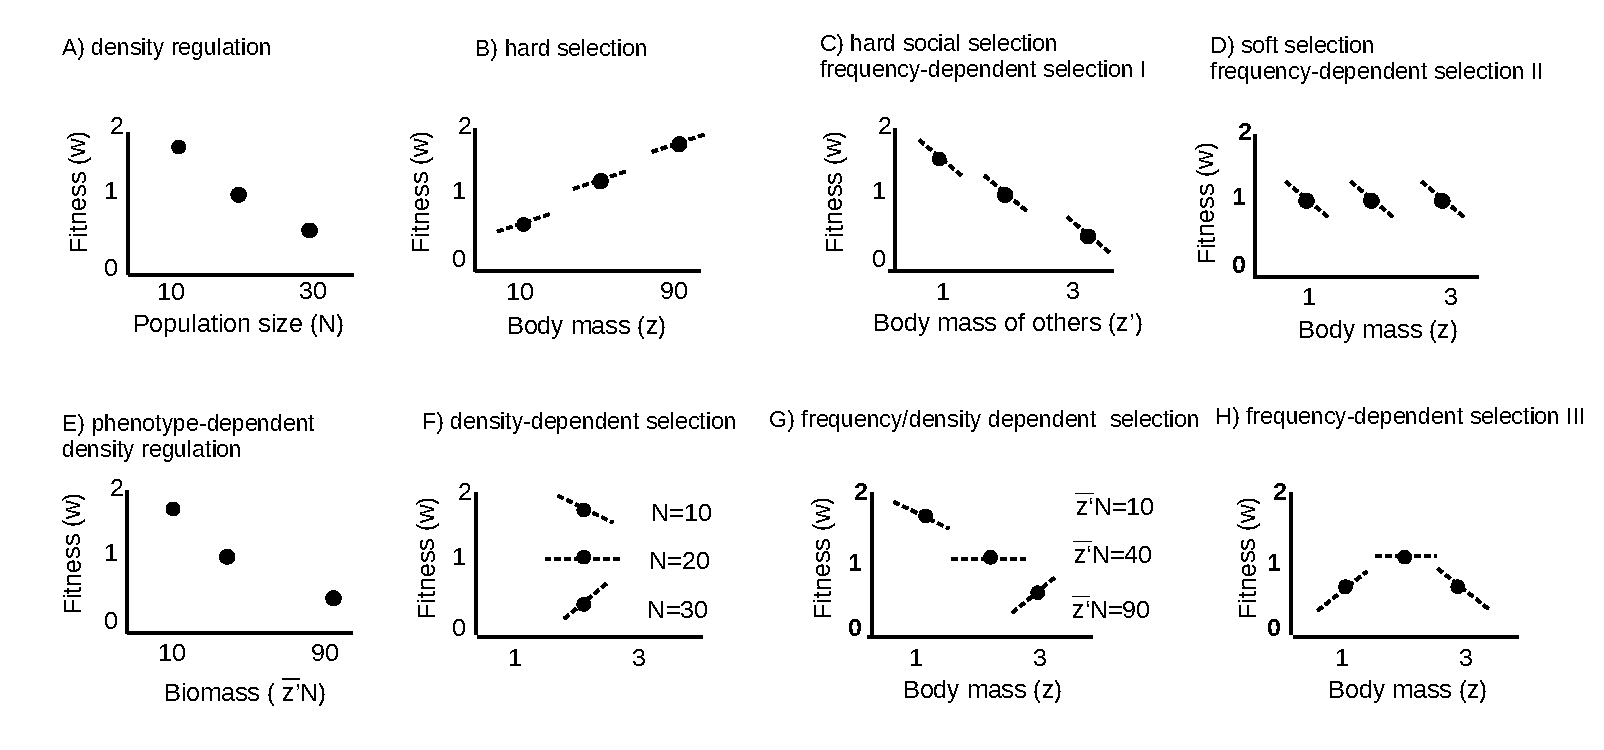
\includegraphics[width=15cm, height=7cm]{Figures/Fig2.pdf}
	\caption{The continuum of social fitness effects on the eco-evolutionary dynamics of populations. Here $w$ is used to denote the fitness of individuals, $z$ their phenotypes, $N$ the number of individuals in the population, and $z’$ the phenotypes of other individuals in the population. While $\bar{z'}$ represents the average phenotype in the social environment. Black dots represent the average phenotype $\bar{z}$ and fitness $\bar{w}$ for a selection episode, and dashed lines represent phenotype-fitness relations within selection episodes. (A) Density regulation, where the number of individuals ($N$) affects the fitness ($w$) of all individuals independent of phenotype. (B) Phenotype-dependent density regulation, where the impact an individual has on the absolute fitness of others depends upon its phenotype, and so in this scenario the effect of population size on fitness ($w$) is moderated by the average phenotype in the population ($\bar{z'}N$). (C) Social selection, where the phenotype of other individuals in the population ($z'$) affects individual absolute fitness ($w$), causing that the mean phenotype in the social environment affects the size of population through its (hard selection) effects on mean fitness. (D) Soft social selection, where the relative fitness ($\frac{w}{\bar{w}}$) of an individual depends on the phenotype of the individuals with whom it interacts (i.e. dashed lines). Note that the assumption that phenotypic effects cause variation only in relative fitness is represented by "forcing" the mean fitness in all selections episodes to be 1 regardless of the mean phenotype in the population (see also scenario D). (E) Density-dependent selection, where the within-episode relationship between an individual's phenotype ($z$) and its absolute fitness ($w$) depends on the number of individuals in the population ($N$) but not on the mean phenotype in the population. (F) Density- and frequency-dependent selection, where the within-episode relationship between an individual's phenotype ($z$) and its absolute fitness ($w$) depends upon both the number of individuals ($N$) and the mean phenotype in the population ($\bar{z}$). (G) Absolute frequency-dependent selection 2, where the relationship between an individual's phenotype and its absolute fitness ($w$) depends upon the mean phenotype in the population ($\bar{z}$), but is independent of the number of individuals in the population ($N$). (H) Classic frequency-dependent selection 3, where the within-episode relationship between an individual's phenotype and its relative fitness ($\frac{w}{\bar{w}}$) depends upon the mean phenotype in the population ($\bar{z}$). The upper panel groups scenarios where the relationship between phenotype and fitness within selection episodes is the same across all selection episodes, and the lower panel groups scenarios where the phenotype-fitness relationship within selection episodes fluctuates across different selection episodes - see main text for further explanation. }
\end{figure}


\begin{figure}[ht]
	\centering
	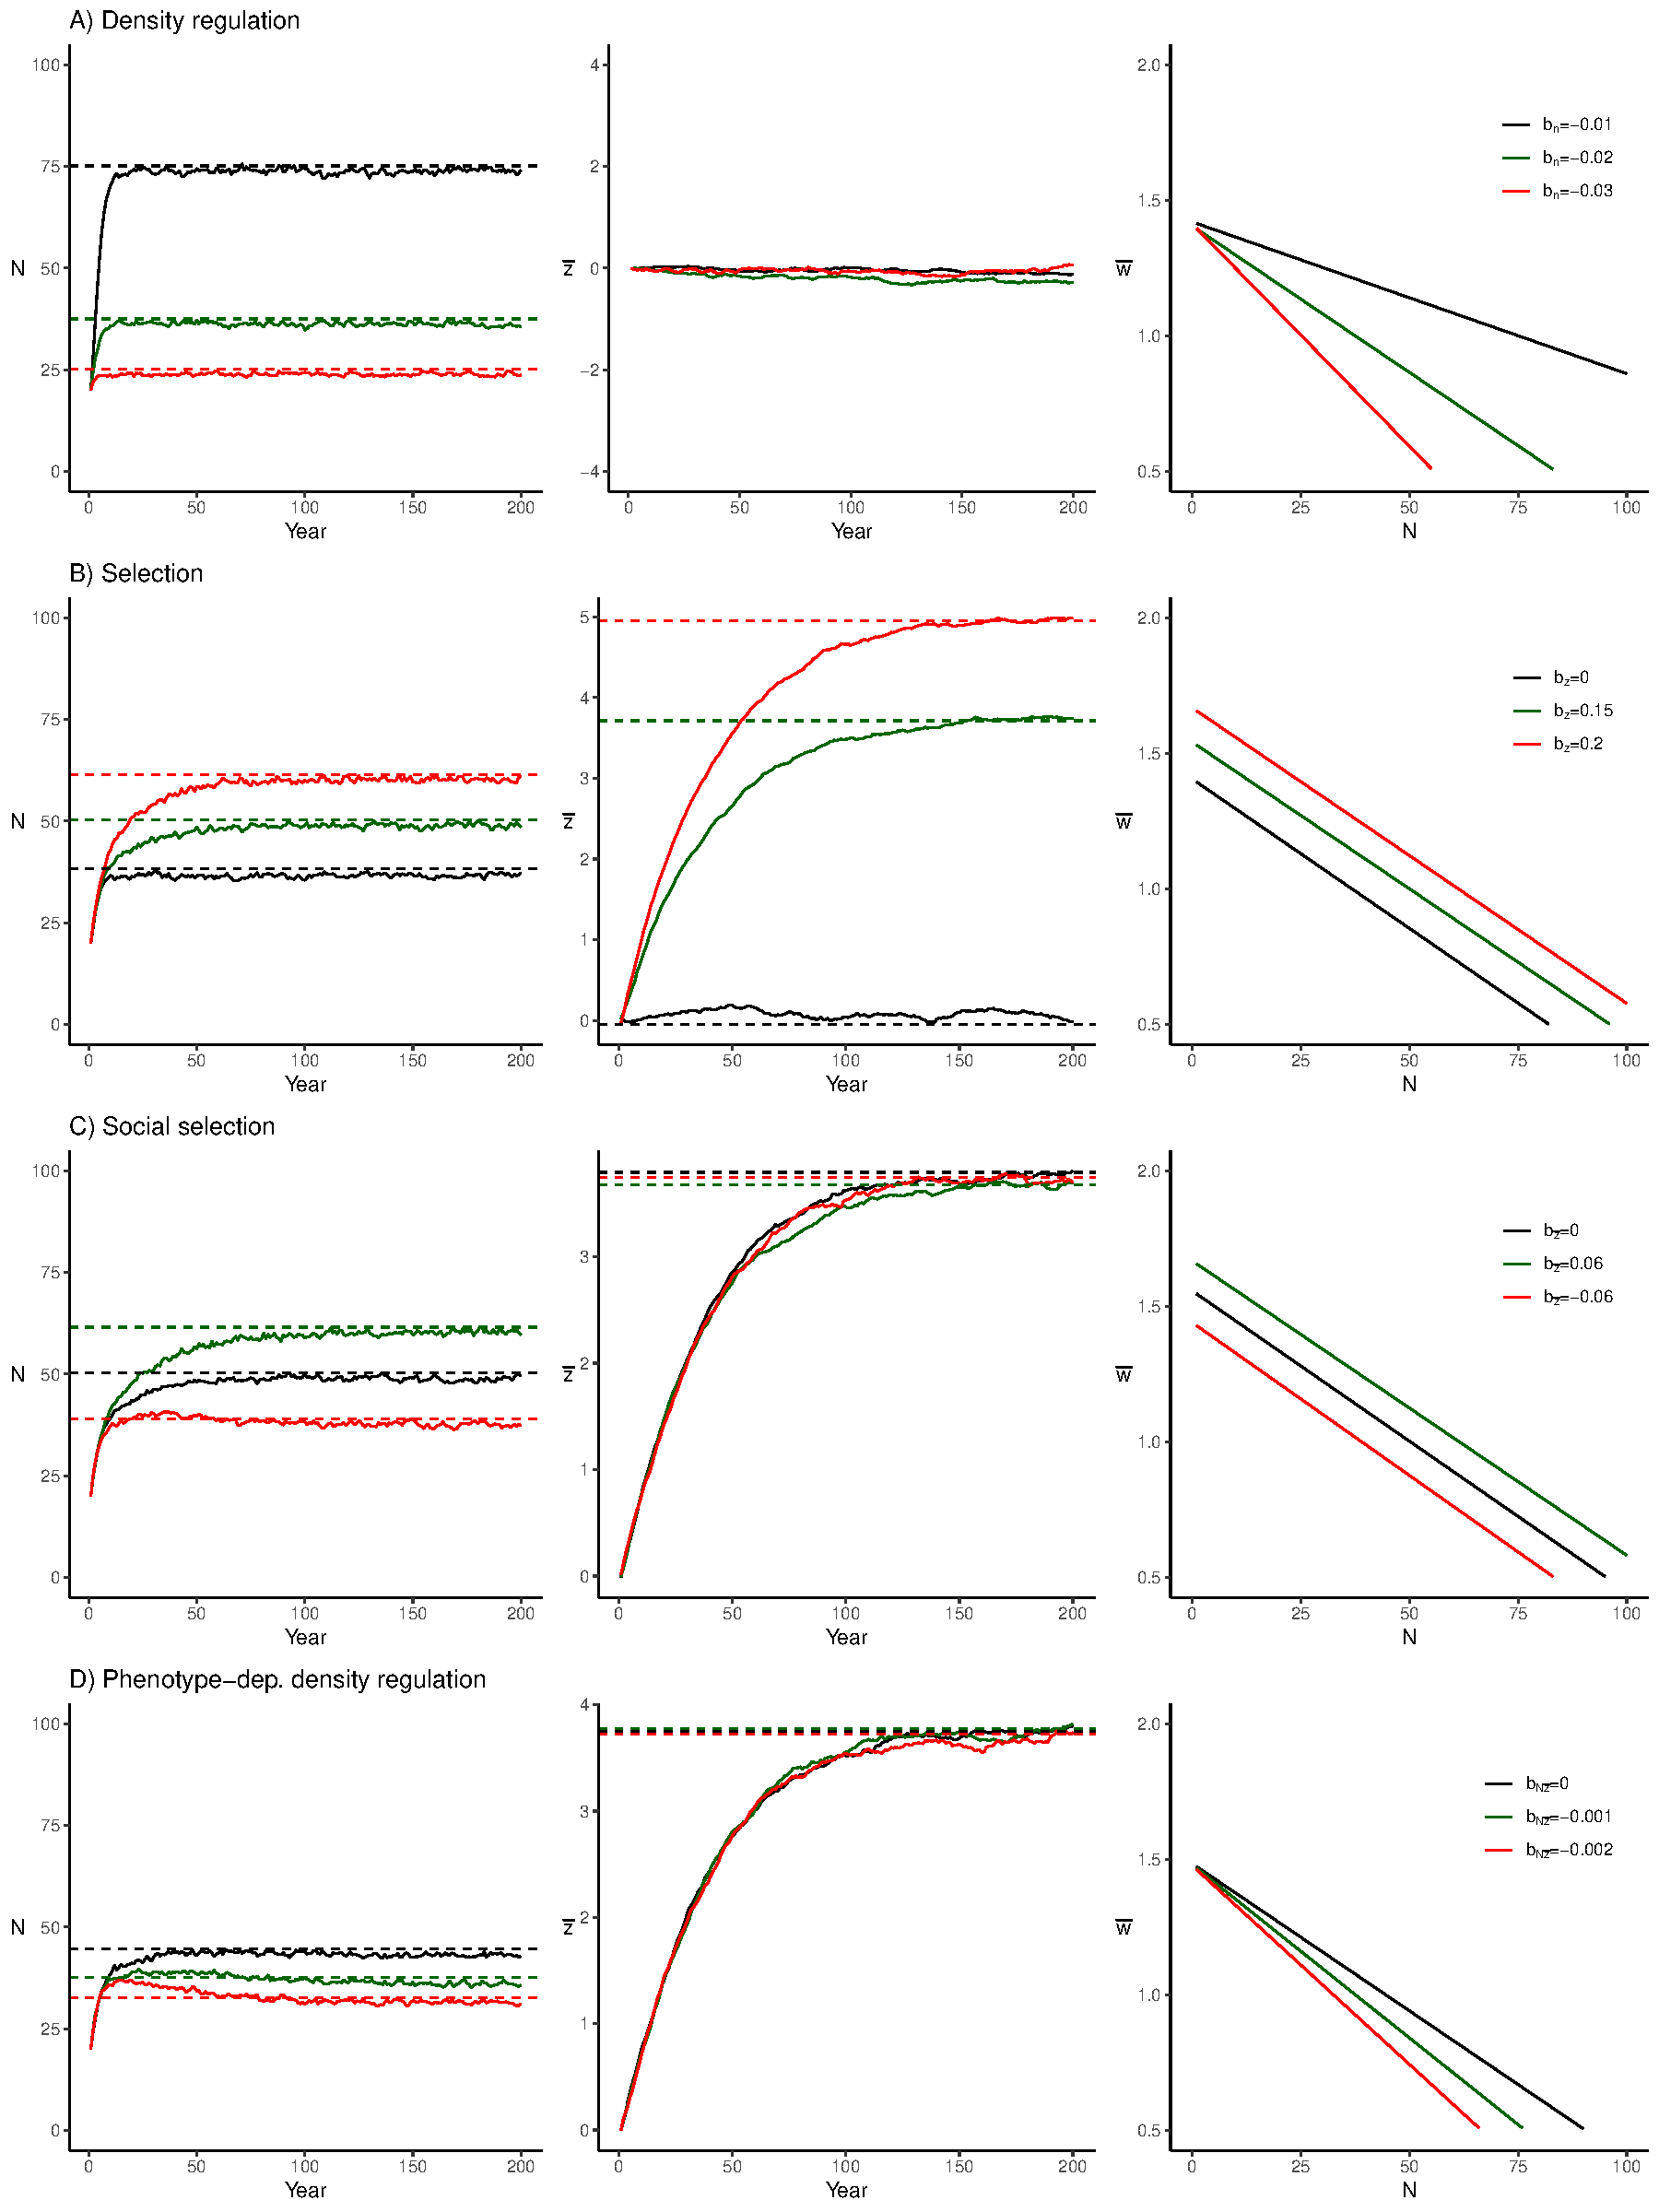
\includegraphics[width=12cm, height=16cm]{Figures/Fig3.pdf}
	\caption{Individual-based simulations results for scenarios of density regulation, direct selection on a phenotype, "hard social selection" and phenotype dependent density regulation. The left-hand graphs show the trajectory of population size until it arrives at its equilibrium, the middle graphs shows the trajectory of the mean phenotype towards its equilibrium, and the right hand graphs shows mean fitness as a function of population size. Lines of different colors represents different parameter values for each scenario. In each scenario we varied a specific parameter, while keeping the other ones constant (see table 2 for simulation parameters). A) Represents a scenario where there is only density regulation and there is no selection on the phenotype. This may reflect a situation where the average phenotype of the population matches the optimum phenotype and there is no phenotypic evolution (middle panel). The different color lines depict how the strength of density regulation (changes in $b_n$ depicted in the right hand side panel) will result in different equilibrium population sizes (left-hand side panel). Panel (B) shows a scenario where there is direct selection on phenotypes, depicting for instance, how a change in the environment (availability of a new resource), results in selection for phenotypes that increase the ability to exploit the new resource. In this scenario the different colored lines represents different strengths of directional selection ($b_z$) on the phenotype. Evolutionary changes are expected to "move" the mean phenotype towards the equilibrium phenotype (middle panel). This will also result in different equilibrium population sizes (left-hand side panel), despite the effect of population size on mean fitness being the same (equal slopes for lines in right-hand side panel). (C) Shows a scenario where the phenotype of individuals in the social environment affect an individual's absolute fitness. The different lines now represent different strength of "hard" social selection ($b_{\bar{z}}$).  The mean phenotype in the social environment affects the equilibrium size of the population (left hand side panel) because it influences the mean fitness of the population, evidenced by the elevation of the population size-fitness relationship in right hand-side panel), even if the equilibrium phenotype is the same (middle panel). Scenario (D) represents a situation where the effect of population size on the average individual fitness depends upon the mean phenotype of the population. The different lines represent different degrees of phenotype dependent density regulation ($b_{N\bar{z}}$), showing that populations with the same mean phenotype (middle panel) can have different equilibrium population sizes (left-hand side panel), when the relation between population size and mean fitness (slope of the population size fitness relation in the right hand side panel) depends on how the mean phenotype modulates the strength of density regulation.}
	\label{fig:sim2}
\end{figure}

\begin{figure}[h] 
	\centering
	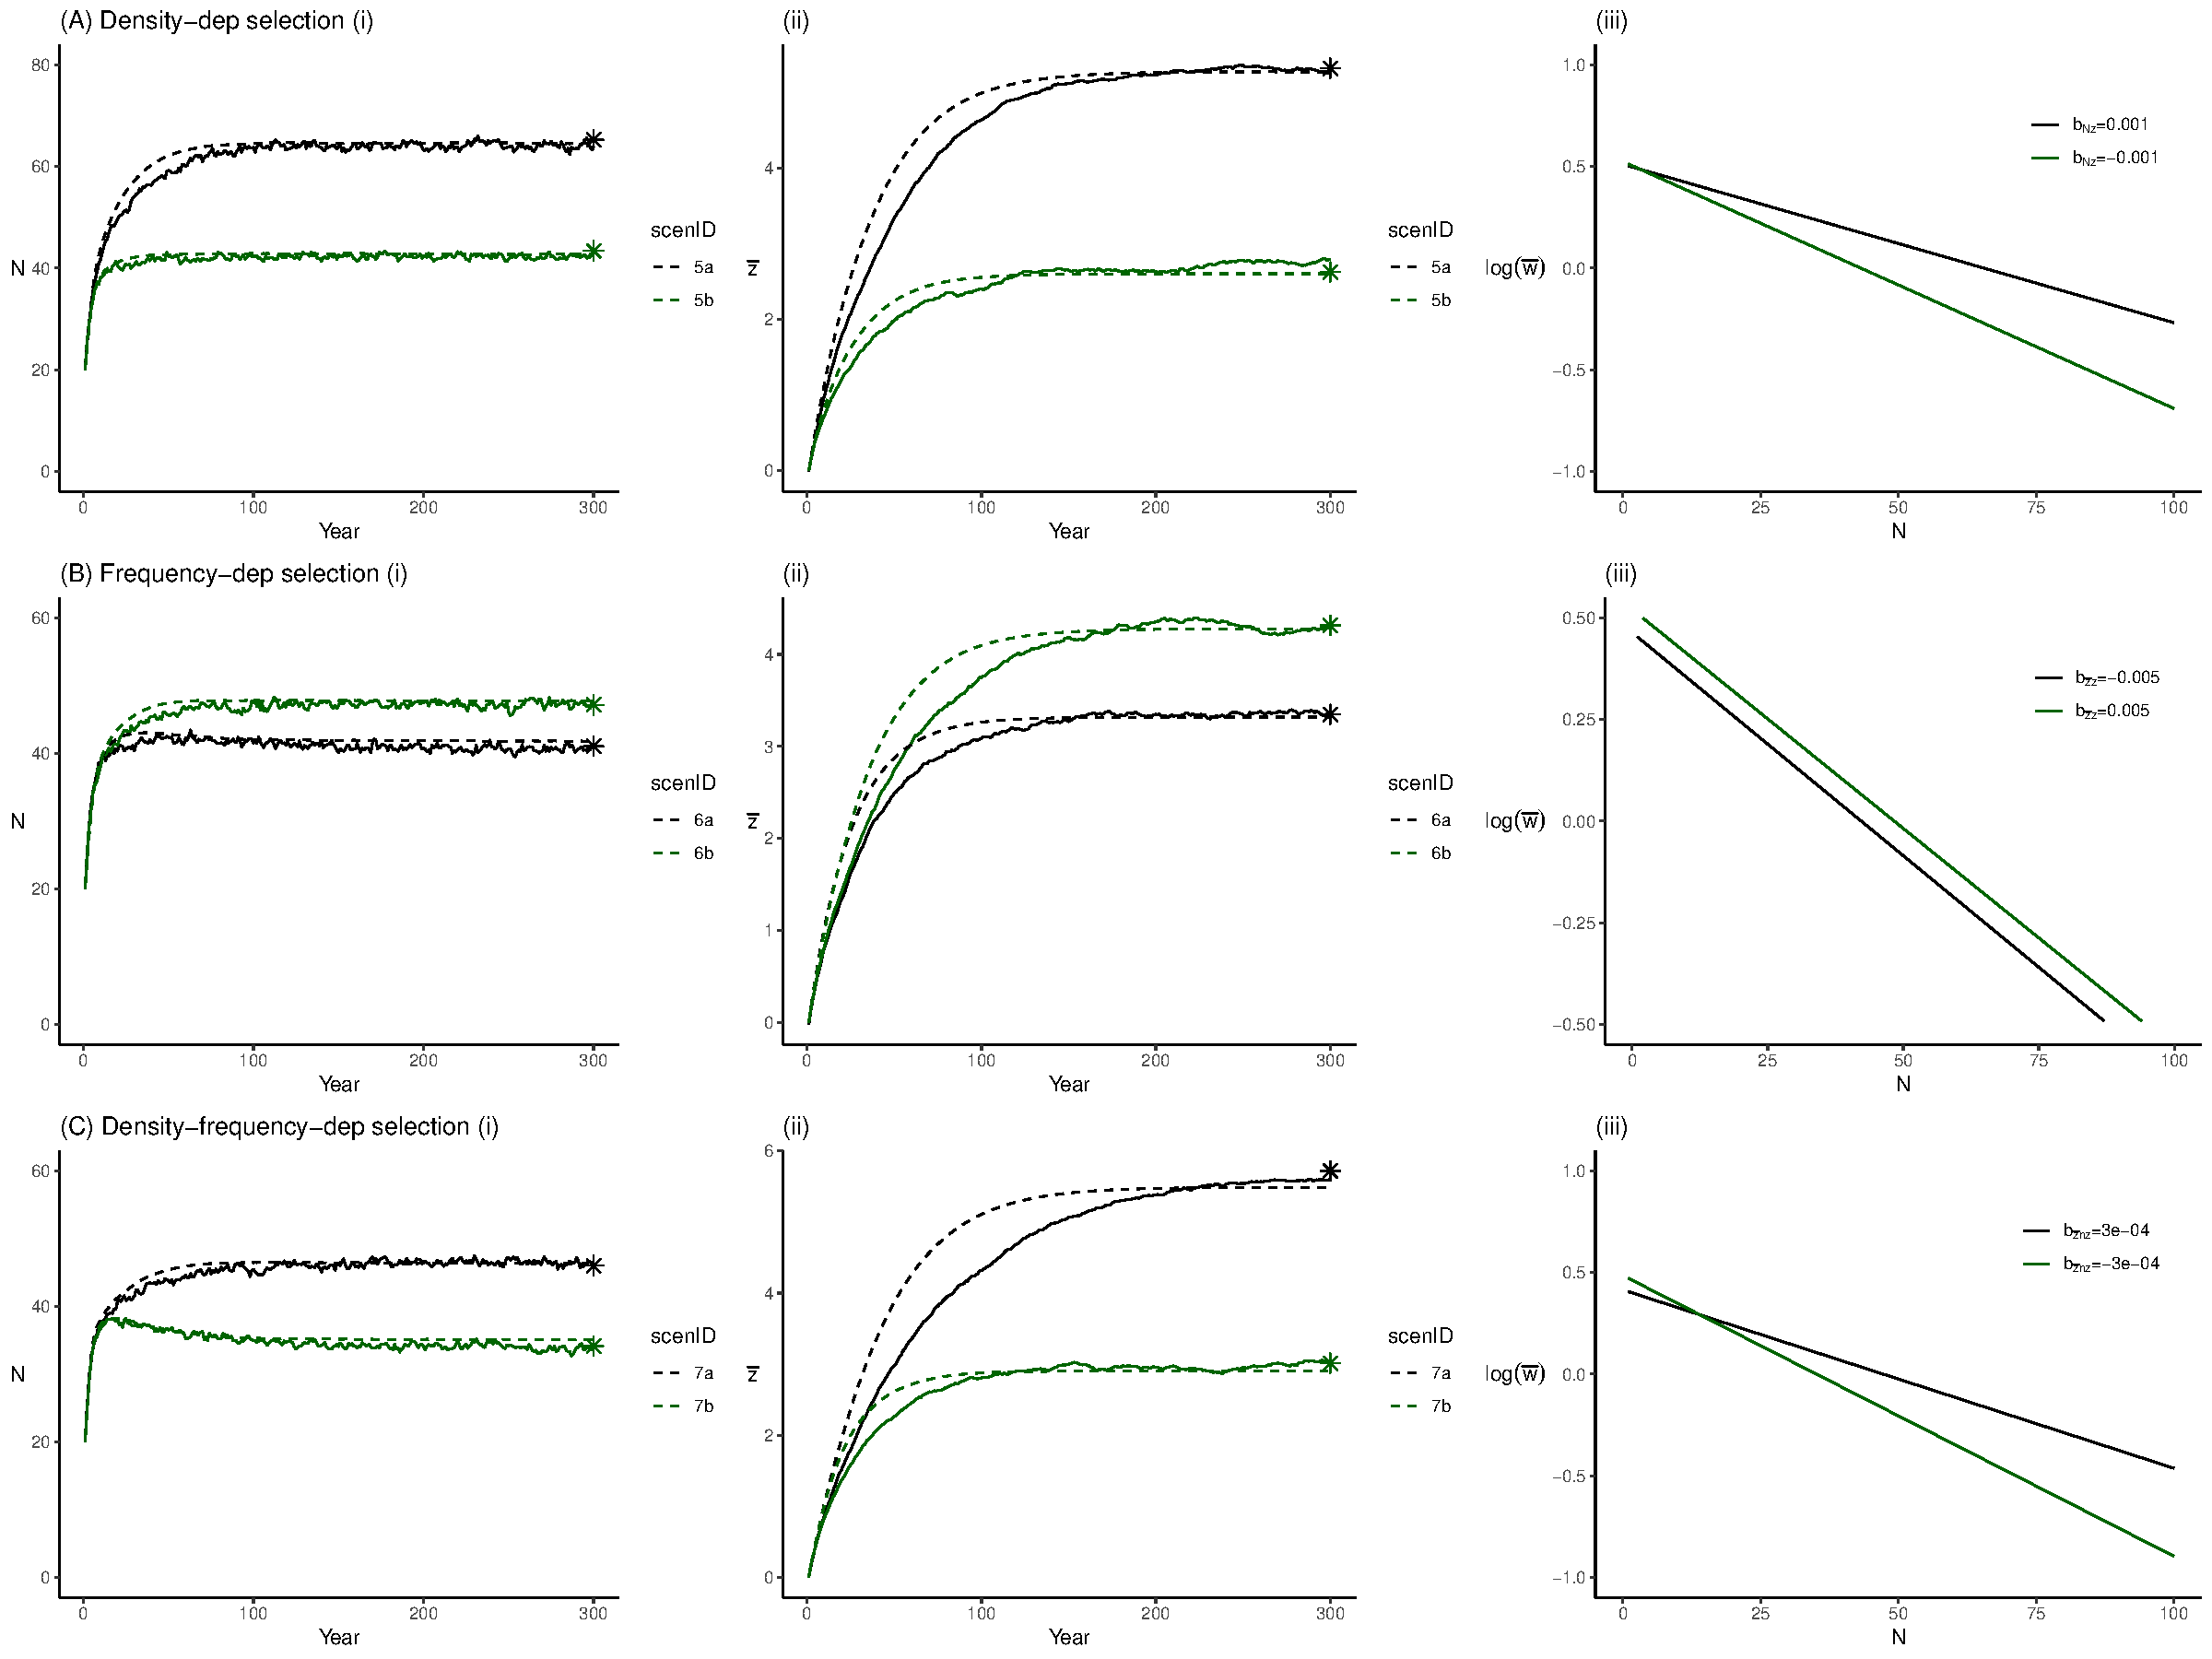
\includegraphics[width=16cm, height=12cm]{Figures/Fig4.pdf}
	\caption{Individual-based simulation results showing the eco-evolutionary consequences of density-dependent selection (A), frequency-dependent selection 2 (B) and their interaction (C). The left-hand side graphs shows the trajectory over time of population size, the middle graphs the trajectory of the mean phenotype, and the right-hand graphs the relationship between the size of the population and its mean fitness. In the simulations of density-dependent selection (A), we varied the density dependent selection coefficient $b_{zn}$, to show how this alters the strength of density regulation (right-hand side graph) and the patterns of selection, with direct consequences to the equilibrium population size (right-hand size) and mean phenotype (middle graph). In the frequency-dependent selection 2  (B), we varied the coefficient $b_{\bar{z}z}$ to show that this has consequences for the expected equilibrium phenotype and also to population size through the effect of the mean phenotype on mean fitness. However, it will not affect the strength of density regulation (right-hand side graph).  When these two process interact resulting in frequency-density-dependent selection (C), the strength of the  coefficeint ($b_{\bar{z}nz}$) will determine the interdependence between the mean phenotype and the equilibrium size of the population. The strength of this coefficeint will affect both the mean fitness of a population when its size is very small and how population size affects the mean fitness of the population (left-hand side panel) which can result in a variety of combinations of equilibrium population size and mean phenotype (see Figure 5).} 
	\label{fig:sim3}
\end{figure}

\begin{figure}[h] 
	\centering
	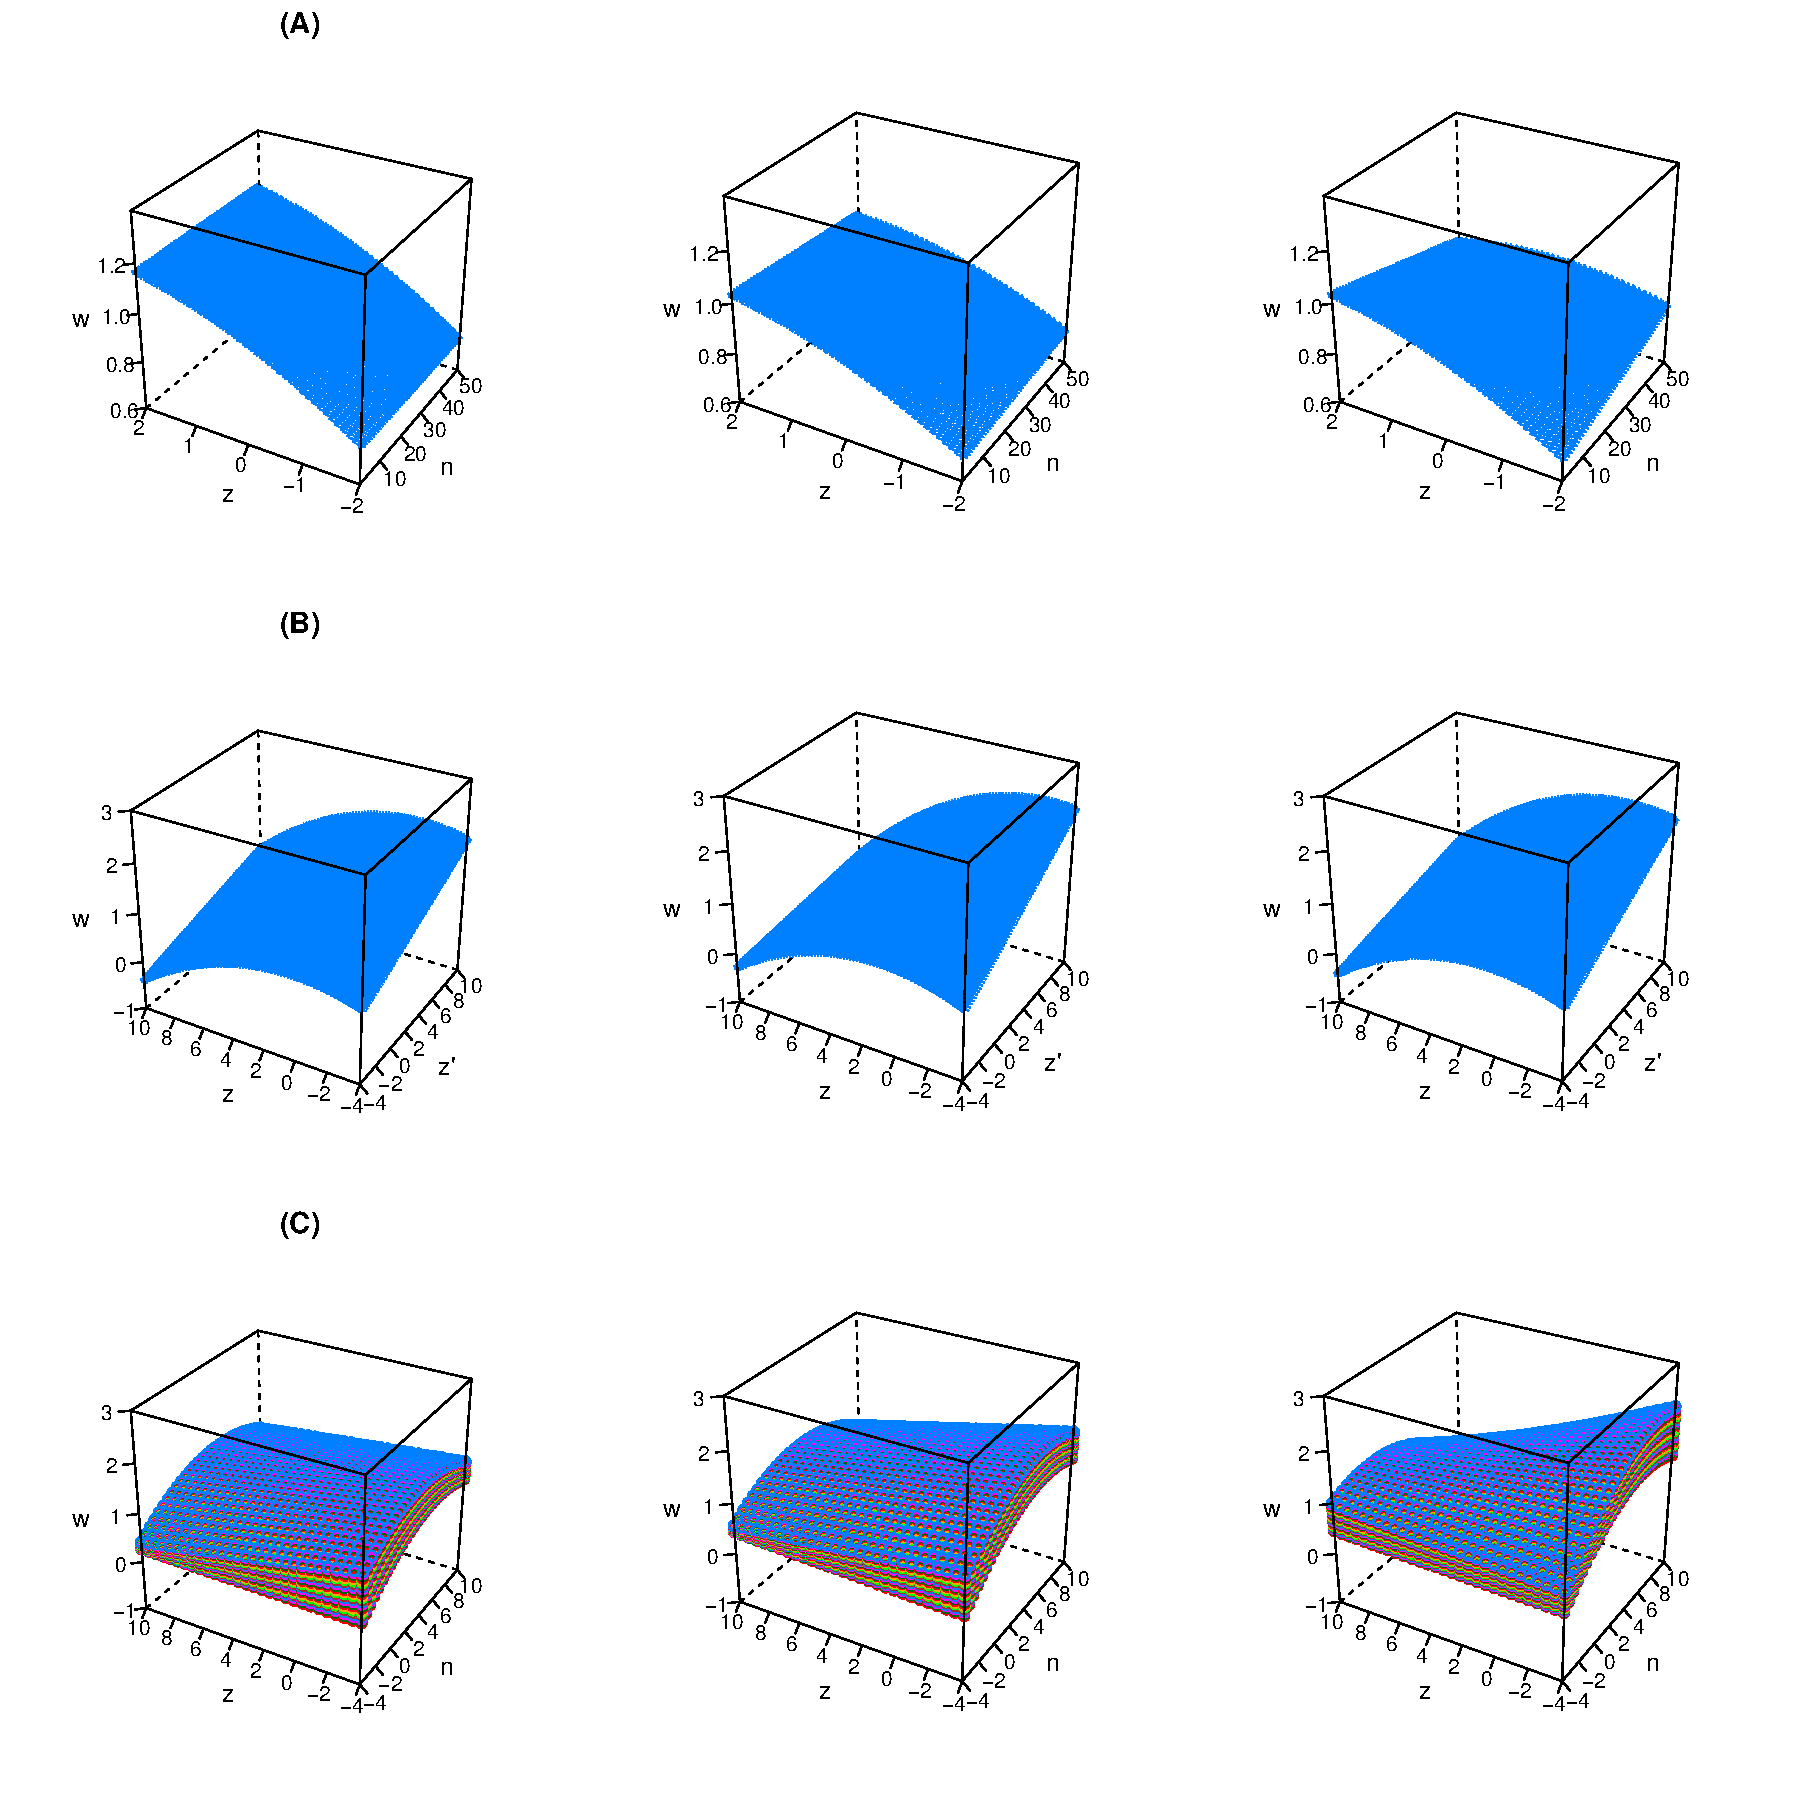
\includegraphics[width=16cm, height=16cm]{Figures/Fig5.pdf}
	\caption{Fitness surface for different scenarios of density-dependent (A), frequency-dependent (B), and frequency-density dependent selection (C). We show relative fitness to emphasize the effects on selection within each episode. The fitness surface corresponds to the predictions based on the multiple regression estimates. Each column represent a different set of simulations with different parameter values for each scenario. In C the different colors represent a different mean phenotype. In this scenario the fitness surface describing the relation between an individuals phenotype, its fitness and the average phenotype in the social environment changes depending on the size of the population.} 
	\label{fig:surface}
\end{figure}



\begin{figure}[h] 
	\centering
	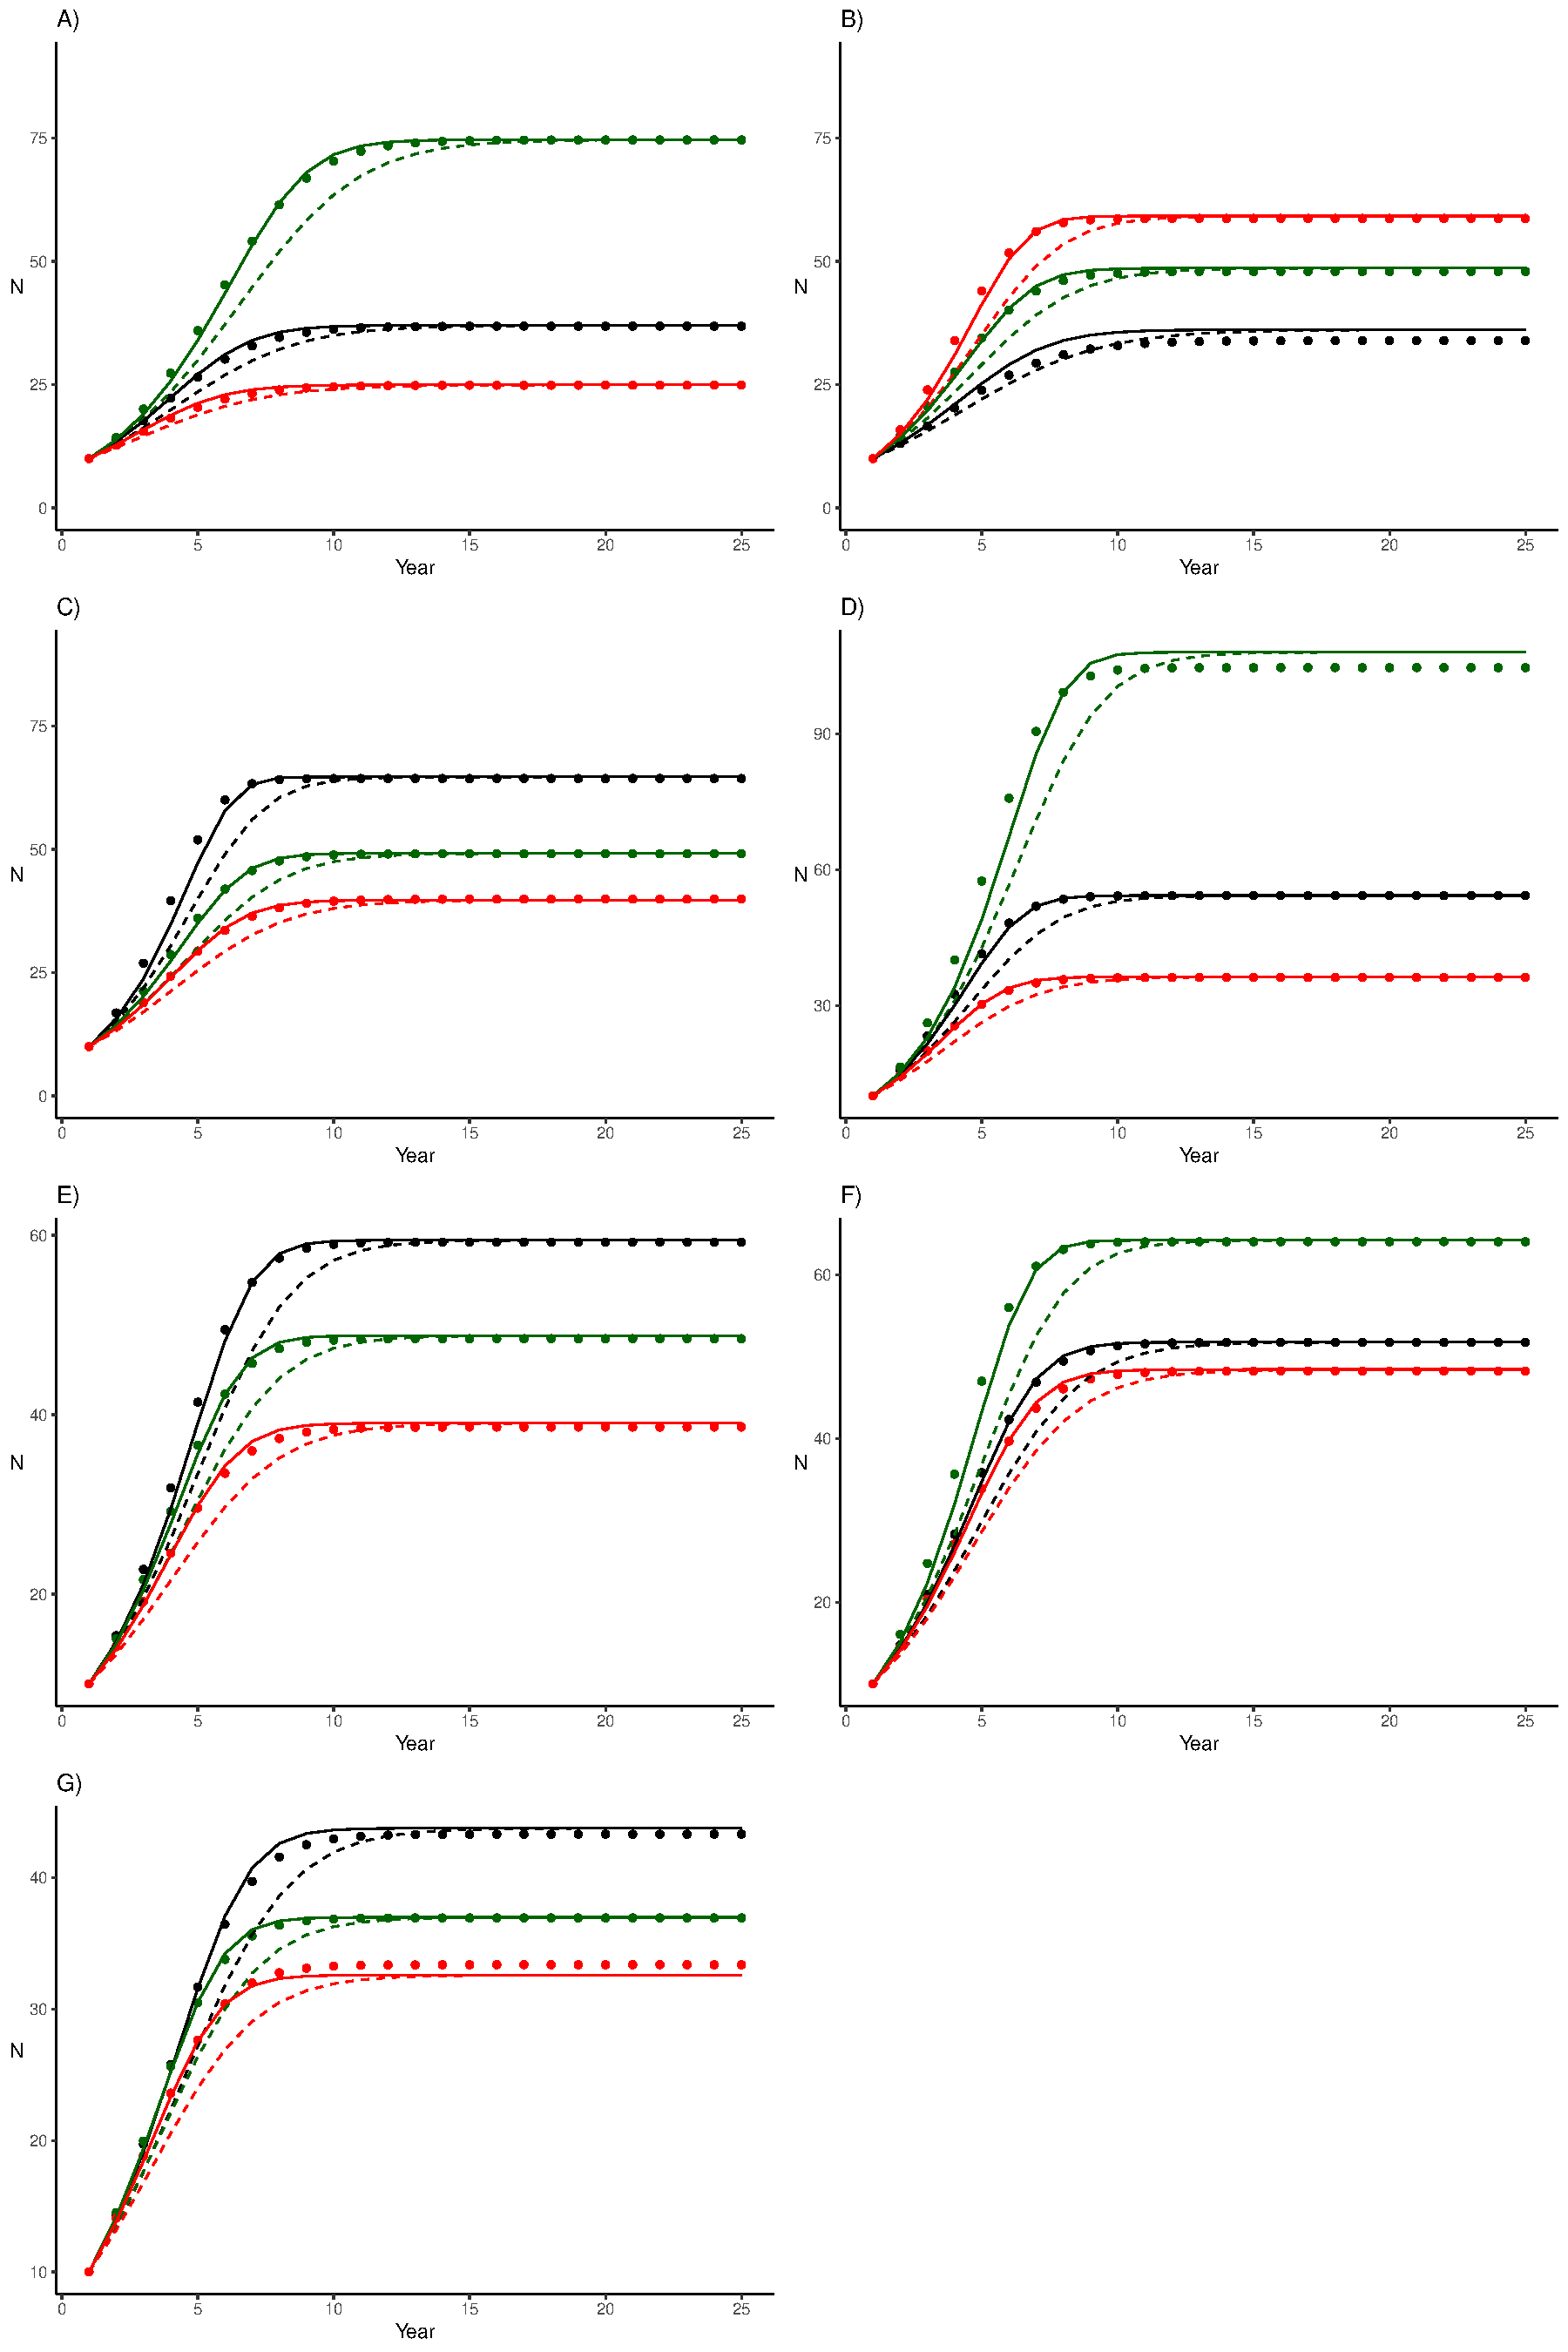
\includegraphics[width=12cm, height=18cm]{Figures/FigS4.pdf}
	\caption{Predicted changes in population size using the multiple regression estimates (circles), a logistic model (dashed lines) and the theta logistic model of population growth (solid line). Colors represent the different simulations for each scenario (see table 2). (A) corresponds to density regulation scenario, (B) to the selection scenario, (C) Social selection scenario, (D) Phenotype dependent regulation, (E) Density dependent-selection, (F) Frequency-dependent selection and (G) Frequency-density-dependent selection} 
	\label{fig:growth}
\end{figure}


 
\end{document}




